%%%%%%%%%%%%%%%%%%%%%%%%%%%%%%%%%%%%%%%%%
% Masters/Doctoral Thesis 
% LaTeX Template
% Version 1.43 (17/5/14)
%
% This template has been downloaded from:
% http://www.LaTeXTemplates.com
%
% Original authors:
% Steven Gunn 
% http://users.ecs.soton.ac.uk/srg/softwaretools/document/templates/
% and
% Sunil Patel
% http://www.sunilpatel.co.uk/thesis-template/
%
% License:
% CC BY-NC-SA 3.0 (http://creativecommons.org/licenses/by-nc-sa/3.0/)
%
% Note:
% Make sure to edit document variables in the Thesis.cls file
%
%%%%%%%%%%%%%%%%%%%%%%%%%%%%%%%%%%%%%%%%%

%----------------------------------------------------------------------------------------
%	PACKAGES AND OTHER DOCUMENT CONFIGURATIONS
%----------------------------------------------------------------------------------------
\documentclass[11pt, oneside]{Thesis-en} % The default font size and one-sided printing (no margin offsets)
\graphicspath{{Pictures/}} % Specifies the directory where pictures are stored
\usepackage[square, numbers, comma, sort&compress]{natbib} % Use the natbib reference package - read up on this to edit the reference style; if you want text (e.g. Smith et al., 2012) for the in-text references (instead of numbers), remove 'numbers' 
\usepackage{amsmath}
\usepackage{caption}
\captionsetup[diagram]{
  justification=raggedright,
  labelsep=newline, % <<< label and text on different lines
  singlelinecheck=false % <<< raggadright also when the caption is shorter
  % than a single line
  }
\captionsetup[figure]{
  justification=raggedright,
  labelsep=newline, % <<< label and text on different lines
  singlelinecheck=false % <<< raggadright also when the caption is shorter
  % than a single line
  }
\captionsetup[table]{
  justification=raggedright,
  labelsep=newline, % <<< label and text on different lines
  singlelinecheck=false % <<< raggadright also when the caption is shorter
  % than a single line
  }
\usepackage{tikz} % for diagrams
\usepackage{imakeidx}\makeindex
\usepackage{hyperref}
\hypersetup{urlcolor=blue, colorlinks=true} % Colors hyperlinks in blue - change to black if annoying
\usepackage{graphicx}
%----------------------------------------------------------------------------------------
\title{\ttitle} % Defines the thesis title - don't touch this
\begin{document}
\frontmatter % Use roman page numbering style (i, ii, iii, iv...) for the pre-content pages
\setstretch{1.3} % Line spacing of 1.3
% Define the page headers using the FancyHdr package and set up for one-sided printing
\fancyhead{} % Clears all page headers and footers
\rhead{\thepage} % Sets the right side header to show the page number
\lhead{} % Clears the left side page header
\pagestyle{fancy} % Finally, use the "fancy" page style to implement the FancyHdr headers
\newcommand{\HRule}{\rule{\linewidth}{0.5mm}} % New command to make the lines in the title page
% Figure size
\newcommand{\myfiguresize}{5.5in}
% PDF meta-data
\hypersetup{pdftitle={\ttitle}}
\hypersetup{pdfsubject=\subjectname}
\hypersetup{pdfauthor=\authornames}
\hypersetup{pdfkeywords=\keywordnames}
%
%----------------------------------------------------------------------------------------
%	TITLE PAGE
%----------------------------------------------------------------------------------------
\begin{titlepage}
\begin{center}
  \textsc{\LARGE \univname}\\[0.5cm] % University name
  \textsc{\Large \facname}\\[1.0cm] % Faculty name
  \textsc{\Large Doctoral Thesis}\\[0.5cm] % Thesis type
  \HRule\\[0.4cm] % Horizontal line
          {\huge \bfseries \ttitle}\\[0.4cm] % Thesis title
          \vfil\textit{2nd unchanged edition in English}
          \HRule\\[1.5cm] % Horizontal line
          \begin{tabular}{l r}
            \parbox{5.5cm}{
              \begin{flushleft}
                \Large\emph{Author:}\\
                \href{http://}{\authornames}
            \end{flushleft}} &
            \parbox{8.5cm}{
              \begin{flushright}
                \Large\emph{Supervisor:} \\
                \href{http://}{\supname}
            \end{flushright}}\\
          \end{tabular}\\[3cm]
          \large\textit{A thesis submitted in fulfilment of the requirements\\ for the degree of \degreename}\\[0.3cm] % University requirement text
          \textit{in the}\\[0.4cm]
          \groupname\\
          \deptname\\[2cm] % Research group name and department name
                     {\large \today}% Date
                     \vfil {(1st ed. April 1991)}\\[3cm]
                     %\includegraphics{Logo} % University/department logo - uncomment to place it
                     \vfill
\end{center}
\end{titlepage}
%----------------------------------------------------------------------------------------
%	DECLARATION PAGE
%	Your institution may give you a different text to place here
%----------------------------------------------------------------------------------------
% \Declaration{
% \addtocontents{toc}{\vspace{1em}} % Add a gap in the Contents, for aesthetics
% \input{Title/EN-Declaration.tex}
% }
% \clearpage % Start a new page

%----------------------------------------------------------------------------------------
%	QUOTATION PAGE
%----------------------------------------------------------------------------------------
%\pagestyle{empty} % No headers or footers for the following pages
%\null\vfill % Add some space to move the quote down the page a bit
%\textit{``Thanks to my solid academic training, today I can write hundreds of words on virtually any topic without possessing a shred of information, which is how I got a good job in journalism."}
%\begin{flushright}
%Dave Barry
%\end{flushright}
%\vfill\vfill\vfill\vfill\vfill\vfill\null % Add some space at the bottom to position the quote just right
%\clearpage % Start a new page

%----------------------------------------------------------------------------------------
%	ABSTRACT PAGE
%----------------------------------------------------------------------------------------
\addtotoc{Abstract} % Add the "Abstract" page entry to the Contents
\abstract{\addtocontents{toc}{\vspace{1em}} % Add a gap in the Contents, for aesthetics
This thesis is devoted to the description of automated working set-up
features for MOS structure evaluation. Using automated HF, LF, QC and
CCT methods the homogeneity of doping profile, lifetime profile,
density of interface states, flatband voltage and oxide thickness was
investigated, with special attention given to the study of MOS
structures with ion-implanted dopants. The homogeneity of investigated
parameters can be depicted by means of two-dimensional color pictures
providing the operator with fast overview of the parameter's
distribution and fluctuations.

}
\clearpage % Start a new page

%----------------------------------------------------------------------------------------
%	ACKNOWLEDGEMENTS
%----------------------------------------------------------------------------------------
\setstretch{1.3} % Reset the line-spacing to 1.3 for body text (if it has changed)
\acknowledgements{\addtocontents{toc}{\vspace{1em}} % Add a gap in the Contents, for aesthetics
\par
I thank my tutor Prof.\ Ing.\ Otto Csabay, PhD. for guidance, valuable
advice, and critical comments in processing of the submitted thesis.

\par
Further I thank the Department of Microelectronics and colleagues from
the Group of electronic components and integrated circuits for
appropriate working conditions and stimulating consultations.

\par
I also thank the staff of Tesla Piešťany, especially RNDr.Boleček, for
testing the homogeneity of specific resistance of silicon wafers
before technological processing and for preparation of samples for the
final experiment.

\par
I thank former colleagues from the Department of Microelectronics
Ing. Ivo Považan and Ing. Tomáš Hrúz for valuable advice and comments
in automation of the experiment and data processing. I thank also
Ing. Ivo Považan for reading the manuscript and for comments on it.

}
\clearpage % Start a new page

%----------------------------------------------------------------------------------------
%	LIST OF CONTENTS/FIGURES/TABLES PAGES
%----------------------------------------------------------------------------------------
\pagestyle{fancy} % The page style headers have been "empty" all this time, now use the "fancy" headers as defined before to bring them back
\lhead{\emph{Contents}} % Set the left side page header to "Contents"
\tableofcontents % Write out the Table of Contents
\lhead{\emph{List of Figures}} % Set the left side page header to "List of Figures"
\listoffigures % Write out the List of Figures
\lhead{\emph{List of Tables}} % Set the left side page header to "List of Tables"
\listoftables % Write out the List of Tables
\clearpage % Start a new page

%----------------------------------------------------------------------------------------
%	ABBREVIATIONS
%----------------------------------------------------------------------------------------
\setstretch{1.5} % Set the line spacing to 1.5, this makes the following tables easier to read
\lhead{\emph{Abbreviations}} % Set the left side page header to "Abbreviations"
\listofsymbols{ll} % Include a list of Abbreviations (a table of two columns)
{
\textbf{CCT} & \textbf{C}onstant \textbf{C}apacity \textbf{T}ime \\
\textbf{CV} & \textbf{C}apacity \textbf{V}oltage \\
\textbf{DLTS} & \textbf{D}eep \textbf{L}evel \textbf{T}ransient \textbf{S}pectroscopy \\
\textbf{GPIB} & \textbf{G}eneral \textbf{P}urpose \textbf{I}nterface \textbf{B}us \\
\textbf{HF} & \textbf{H}igh \textbf{F}requency \\
\textbf{LF} & \textbf{L}ow \textbf{F}requency \\
\textbf{MOS} & \textbf{M}etal \textbf{O}xid \textbf{S}emiconductor \\
\textbf{SIMS} & \textbf{S}econdary \textbf{I}on \textbf{M}ass \textbf{S}pectrometry
\\ [1.0cm]
\textbf{SCR} & \textbf{S}pace \textbf{C}harge \textbf{R}egion
%\textbf{Acronym} & \textbf{W}hat (it) \textbf{S}tands \textbf{F}or \\
}

\clearpage % Start a new page

%----------------------------------------------------------------------------------------
%	PHYSICAL CONSTANTS/OTHER DEFINITIONS
%----------------------------------------------------------------------------------------
\lhead{\emph{Physical Constants}} % Set the left side page header to "Physical Constants"
\listofconstants{lrcl} % Include a list of Physical Constants (a four column table)
{
Boltzmann constant & $k$ & $=$ & $1.38\times10^{-23}\mbox{JK}^{\mbox{-1}}$ \\
Intrinsic concentration of charge carriers in silicon & $n_i$ & $=$ & $1.45\times10^{16}\mbox{m}^{\mbox{-3}}$ \\
Electron charge & $q$ & $=$ & $1.602\times10^{-19}\mbox{C}$ \\
$\beta$ & $\beta$ & $=$ & ${q}/{kT}$
% Constant Name & Symbol & = & Constant Value (with units) \\
}

\clearpage % Start a new page

%----------------------------------------------------------------------------------------
%	SYMBOLS
%----------------------------------------------------------------------------------------
\lhead{\emph{Symbols}} % Set the left side page header to "Symbols"
\listofnomenclature{lll} % Include a list of Symbols (a three column table)
{
% Symbol & Name & Unit \\
$A$ & MOS structure area & $m^2$ \\
$C$ & Capacitance & $F$ \\
$C_{i}$ & capacitance of voltage-independent capacitor Q-C method & $F$ \\
$C_{iHF}$ & HF capacitance of voltage-independent capacitor of Q-C method & $F$ \\
$C_{iLF}$ & LF capacitance of voltage-independent capacitor Q-C method & $F$ \\
$C_{m}$ & LF capacitance of series-parallel circuit of Q-C method & $F$ \\
$C_{mos}$ & differential capacitance of MOS structure & $F$ \\
$C_{mos}^{HF}$ & high frequency capacitance of MOS structure & $F$ \\
$C_{mos}^{LF}$ & low frequency capacitance of MOS structure & $F$ \\
$C_{mos}^{TLF}$ & theoretical low frequency capacitance of MOS structure & $F$ \\
$C_{ox}$ & oxide layer capacitance of MOS structure & $F$ \\
$C_{sc}$ & space charge region capacitance & $F$ \\
$C_{w}$ & parasitic capacitance of Q-C method & $F$ \\
$C_{x}$ & parasitic capacitance of Q-C method & $F$ \\
$D$ & dose of implanted atoms in the semiconductor & $m^{-2}$ \\
$D_{i}$ & dose of implanted atoms specified in the implantation process & $m^{-2}$ \\
$D_{it}$ & trap density of the $Si-SiO_2$ interface & $m^{-2}eV^{-1}$ \\
$D_{n}$ & electron diffusion coefficient & $m^{-2}s^{-1}$ \\
$E$ & energy & $eV$ \\
$E_{c}$ & energy of the lower edge of the conduction band & $eV$ \\
$E_{f}$ & Fermi level energy in the semiconductor & $eV$ \\
$E_{i}$ & energy of the intrinsic Fermi level in the semiconductor & $eV$ \\
$E_{v}$ & energy of the upper edge of the valence band & $eV$ \\
$G_{m}$ & conductivity of series-parallel connection of Q-C method capacitors & $F$ \\
$h_{ox}$ & oxide layer thickness of MOS structure & $m$ \\
$I,i$ & electric current & $A$ \\
$I_{g}$ & generation current of minority charge carriers & $A$ \\
$L_{D}$ & Debay length & $m$ \\
$L_{DE}$ & extrinsic Debay length & $m$ \\
$N$ & concentration of interacting impurities in the semiconductor & $m^{-3}$ \\
$n$ & concentration of electrons in the semiconductor & $m^{-3}$ \\
$N_{A}$ & concentration of acceptors & $m^{-3}$ \\
$N_{b}$ & substrate concentration & $m^{-3}$ \\
$N_{D}$ & donor concentration & $m^{-3}$ \\
$N_{\max}$ & maximum concentration of dopants in the semiconductor & $m^{-3}$ \\
$P$ & concentration of holes in the semiconductor & $m^{-3}$ \\
$Q$ & electric charge & $C$ \\
$Q_{dc}$ & breakdown charge in $SiO_2$ and at the semiconductor-metal interface & $C$ \\
$R_{p}$ & mean value of the distribution of implanted atoms in the semiconductor & $m$ \\
$\Delta R_{p}$ & variance of the distribution of implanted atoms in the semiconductor & $m$ \\
$T$ & temperature & $K$ \\
$t$ & time & $s$ \\
$u$ & normalized electric potential in the semiconductor & \\
$u_f$ & normalized Fermi potential in the semiconductor & \\
$u_s$ & normalized potential at the semiconductor surface &  \\
$V$ & voltage & $V$ \\
$V_a$ & voltage on series-parallel connection of Q-C method capacitors & $V$ \\
$V_{fb}$ & voltage of aligned strips of MOS structure & $V$ \\
$V_{g}$ & gate electrode voltage of MOS structure & $V$ \\
$V_i$ & voltage at the common point of the series-parallel Q-C method & $V$ \\
$V_{ox}$ & voltage drop across the oxide layer of the MOS structure & $V$ \\
$w$ & width of space charge region & $m$ \\
$x$ & distance & $m$ \\
$\overline z$ & mean value of random variable z & \\
$\delta z$ & variance of random variable z & \\
$z^{'}$ & spatial derivative of random variable z & \\

& & \\% Gap to separate the Roman symbols from the Greek
\newpage
$\epsilon$ & permittivity & $Fm^{-1}$ \\
$\epsilon_s$ & permittivity $Si$ & $Fm^{-1}$ \\
$\epsilon_{ox}$ & permittivity $SiO_2$ & $Fm^{-1}$ \\
$\varphi$ & electric potential & $V$ \\
$\varphi_{ms}$ & output potential difference between metal and semiconductor & $V$ \\
$\varphi_{s}$ & voltage drop across the semiconductor layer (surface potential) & $V$ \\
$\mu_{n}$ & electron mobility in the semiconductor & $m^2V^{-1}s^{-1}$ \\
$\mu_{p}$ & mobility of holes in the semiconductor & $m^2V^{-1}s^{-1}$ \\
$\omega$ & angular frequency & $s^{-1}$ \\
$\tau_g$ & generation time of minority charge carriers & $s$ \\

% Symbol & Name & Unit \\
}

\clearpage % Start a new page

%----------------------------------------------------------------------------------------
%	DEDICATION
%----------------------------------------------------------------------------------------
%\setstretch{1.3} % Return the line spacing back to 1.3
%\pagestyle{empty} % Page style needs to be empty for this page
%\dedicatory{\input{Title/Dedication.tex}} % Dedication text
%\addtocontents{toc}{\vspace{2em}} % Add a gap in the Contents, for aesthetics
%\clearpage % Start a new page

%----------------------------------------------------------------------------------------
%	INTRODUCTION
%----------------------------------------------------------------------------------------
\setstretch{1.3} % Return the line spacing back to 1.3
\pagestyle{fancy} % Return the page headers back to the "fancy" style
\input{Chapters/EN-Introduction}
\addtocontents{toc}{\vspace{2em}} % Add a gap in the Contents, for aesthetics

%----------------------------------------------------------------------------------------
%	THESIS CONTENT - CHAPTERS
%----------------------------------------------------------------------------------------
\mainmatter% Begin numeric (1,2,3...) page numbering
\pagestyle{fancy} % Return the page headers back to the "fancy" style
% Include the chapters of the thesis as separate files from the Chapters folder
% Uncomment the lines as you write the chapters
% Chapter 1
% Main chapter title
\chapter{The current state of the subject.}% For referencing the chapter elsewhere, use \ref{Chapter1}
\label{Chapter1}
% This is for the header on each page - perhaps a shortened title
\lhead{Chapter 1. \emph{The current state of the subject}} 

Up to now, the methods used for analysis of electrophysical properties
of MOS structures are based on the assumption that the distribution of
impurities in the substrate is homogeneous. This issue was addressed
by the Department of Microelectronics within the government research
projects~\cite{1.1,1.2} and PhD thesis~\cite{1.5,1.6,1.7,1.8}. These
works provide the necessary overview of the solutions for the problems
globally and also in our department. Whereas at present in the
manufacture of unipolar integrated circuits using ion implantation for
control the electrical properties of integrated components, it is
desirable to control the properties of semiconductor structures to
know the parameters of MOS structures with inhomogeneous subsidy
substrate. For this purpose was research task Electrophysical
properties of microelectronic structures~\cite{1.3,1.4} focused on the
development of diagnostic methods for study of the properties of
technological processes using MOS structures with inhomogeneous
subsidy impurities and their application to solving problems of
Czech-Slovak semiconductor industry. From this target of the government
research project resulted the focus of the presented thesis. The need
to address this issue is also based on the fact that up till now this
issue, as far as we known, has never been studied here. Additionally,
the issue was extended to the research of electro-physical parameters'
homogeneity of MOS structures on silicon substrate, which is
particularly serious in the light of the process quality improvement
of forming a semiconductor structures and integrated circuits by
planar technology. Based on the foregoing, we list later in this
chapter only the most necessary knowledge needed to deal with the
issues.

\section{Basics of the MOS structure.}

MOS structure forms a simple test structure. Almost all of its
electrical properties can be examined by measurements of this
structure. Convenience of the MOS structure lies in the ease of
preparation and analysis of its features. The simplicity of analysis
follows that analyzed system is in thermal equilibrium and
one-dimensional approach is sufficiently accurate in most
cases. Properties of the $SiO_2$ volume, its interfaces with
semiconductor and metal, as well as properties of the subsurface area
of semiconductor can be examined by electrical measurements of MOS
structure.

\section{Ideal MOS structure.}\index{MOS!ideal structure}

MOS structure can be considered a dipole, which equivalent scheme can
be thought of as a serial connection of voltage-independent capacity
of the oxide $C_{ox}$ and capacity of the space charge region (SCR)
$C_{sc}(\varphi_{s})$, which is a function of the surface potential of
the semiconductor. Then for the capacity of MOS structure is
valid~\cite{I.1}

\begin{equation}\label{eq:1.1}
  \frac{1}{C_{mos}(V_g)} = \frac{1}{C_{ox}} + \frac{1}{C_{sc}(\varphi_s)}
\end{equation}

Following simplistic assumptions, that define ideal MOS structure, can
be used when analyzing the MOS structure:

\begin{itemize}
\item the density of interface traps $Si-SiO_2$ is equal zero
\item there are no charges in the insulator $SiO_2$
\item the difference in the output potential of the metal and
  semiconductor is equal zero
\item equation $V_{g}=V_{ox}+\varphi_{s}$ is valid.
\end{itemize}

\noindent Depending on the gate voltage operating modes of MOS
structure can be distinguished:

\begin{itemize}
\item enhancement mode
\item flat band mode
\item depletion mode and inversion (deep depletion).
\end{itemize}

\section{Capacitor characteristics of ideal MOS structure.}\index{MOS!ideal structure}

For all of these cases one-dimensional Poisson equation is valid in
the semiconductor

\begin{equation}\label{eq:1.2}\index{Poisson equation}
  \frac{d^2\varphi}{dx^2} = -\frac{q}{\varepsilon}(p-n+N_{p}-N_{A})
\end{equation}

which determines the course of the electrical potential $\varphi$ as a
function of the distance from the surface of the semiconductor
$x$. Equation~\ref{eq:1.2} can be solved analytically only for certain
special cases of the impurities concentration profile, and, in
general, numerical methods must be used~\cite{1.9,1.10}. Then, for
known profile of the concentration impurities in semiconductor an
electric potential in the semiconductor can be obtained, where
potential on the gate is the parameter which defines the state of the
MOS structure. For further clarification of physical processes in the
MOS structure in the transition from accumulation to inversion, or
deep depletion, we solved the equation~\ref{eq:1.2}, where by
appropriate variation of the parameter $V_g$ both surface
potential~\index{surface potential} $\varphi_{s}(V_g)$ and capacity of
MOS structure $C_{MOS}(V_g)$ can be calculated as a function of the
gate voltage (see Appendix~\ref{app:AppendixA}).

\begin{figure}[h!]\centering
  \includegraphics{Figures/fig-1-1.eps}% chktex-file 8
  \caption[Concentration of dopant in the subsurface of the
    semiconductor] {Concentration of dopant in the subsurface of the
    semiconductor simulated by Gaussian distribution~\cite{1.11} with
    the following parameters $R_p=0.1 \mu{m}$;
    $\Delta{R_p}=0.03\mu{m}$; $N_{\max}=10^{23} m^{-3}$;
    $N_{bulk}=10^{20} m^{-3}$ (indicated by a solid line 1). The
    profile of the majority charge carriers for $V_g=0$ (indicated by
    a solid line 2). The dotted line shows profiles of the
    concentrations of majority carriers for various gate voltages
    different from zero. State of thermodynamic equilibrium between
    the distribution of dopant and charge carriers is described in
    Appendix~\ref{app:AppendixD}.}\label{fig:1.1}
\end{figure}

\par Figure~\ref{fig:1.1} shows the profile of the dopant
concentration in semiconductor (simulated by Gaussian function) and
profiles of majority charge carriers for states of the structure
varying from enhancement to inversion, depicting the process of
depletion of the semiconductor subsurface. It can be seen, that the
profile of the concentration of majority carriers in implanted field
enter the maximum and then decreases toward the concentration of the
substrate, which is reached at a ground potential point. Also obvious
is the difference between the concentrations of dopant and the
concentration of majority charge carriers in the state of
thermodynamic equilibrium for zero gate voltage, which results indue
to diffusion of majority charge carriers.

\newpage
\begin{figure}[h!]\centering
  \includegraphics{Figures/fig-1-2.eps}
  \caption[Surface potential $\varphi_s(V_g)$ as a function of the
    gate voltage]{Surface potential $\varphi_s(V_g)$ as a function of
    the gate voltage for low frequency (LF) and high frequency (HF)
    measurement (depicted 1) and measurement in deep depletion
    (depicted 2).}\label{fig:1.2}
\end{figure}

\begin{figure}[h!]\centering
  \includegraphics{Figures/fig-1-3.eps}
  \caption[Profile of the capacity of the MOS structure depending on
    the gate voltage]{Profile of the capacity of the MOS structure
    depending on the gate voltage for low frequency measurement
    (depicted 1), high frequency measurement (depicted 2) and
    measurement in deep depletion (depicted 3).}\label{fig:1.3}
\end{figure}

\par Figure~\ref{fig:1.2} shows surface potential for various
measurements of the MOS structure. In the enhancement and depletion
both curves are identical. From the beginning of the inversion the
surface potential stabilizes for LF and HF measurements as a result of
the creation of the inversion layer. The curve of deep depletion
further declines. This state will be terminated by the breakdown in a
real structure.

\par Figure~\ref{fig:1.3} shows Capacitance-Voltage profiles of the
MOS structure. All three curves are identical in enhancement and
depletion (profiles of the surface potential are also identical). In
this section the capacity declines slowly, because the space charge
region expands to the region with high concentration of the
dopant~\ref{fig:1.1}. From the beginning of the inversion the the
curves depart. Low frequency curve, which detects the inversion layer
rises toward the capacity of the silica. High frequency curve doesn't
detect the inversion layer, because the minority charge carriers are
not able to follow the high frequency measurement signal. However the
capacity doesn't decline any further, because with the increasing of
the gate voltage increases mostly the concentration of the minority
charge carriers in the inversion layer and the space charge region
doesn't expand any further.

\par No inversion layer is created in deep depletion and with the
increasing gate voltage the space charge region expands and capacity
declines. Figure~\ref{fig:1.3} shows, that after having passed the
section with the high concentration of dopant the curve of deep
depletion starts to decline faster.

\section{Real MOS structure.}\index{MOS!real structure}

The difference of ideal and real MOS structure was treated
in~\cite{1.12} and here we introduce only a review. Electrical
properties of real MOS structure are different from the ideal model
mainly due to the defect charges in the oxide layer and in its
interface with the semiconductor and metal, which can be divided into
the following groups:

\begin{itemize}
\item charge of the mobile ions in the oxide layer - $Q_{m}$
\item charge of the ionized traps in the oxide - $Q_{ox}$
\item fixed charge at the interface $Si-SiO_2$, due to the
  non-stoichiometric composition of the phase transition - $Q_f$
\item charge of the traps at the interface $Si-SiO_2$ - $Q_{it}$
\end{itemize}

\par At the same time the electrical properties of MOS structure are
also affected by the difference in work function between metal and
semiconductor, $\varphi_{ms}\neq{0}$. In addition to the defect
charges geometrical imperfections of the structure, changing thickness
of the insulating layer and non-planarity of the interface $Si-SiO_2$
influence electrical properties of MOS structure. The transition to a
very large integration requires to address the micro-defects in the
volume of silicon, which represent a disorder of the crystal lattice
resulted in the production of the mono-crystal, its primary treatment
to the form of a silicon wafer and during the technological processing
of the components. If those defects are found in the area of
functional parts, they have adverse effects on electrical
parameters. However, micro-defects of suitable size in the volume of
semiconductor produce effects which are often used to create so-called
denuded zone. Deliberate creation of micro-defects in the volume of
semiconductor by implantation of carbon and subsequent heating may
significantly increase the lifetime of the minority charge
carriers~\cite{1.13}. In~\cite{1.14} authors clearly displayed with
laser scanning tomography a denuded zone at silicon surface formed by
microprecipitates $SiO_x$. Microprecipitates in the volume of the
semiconductor, created with oxygen and appropriate heat-processing,
are also seen from the images.

\begin{thebibliography}{}
\bibitem[1.1]{1.1} Csabay O. et al: Výskum štruktúr MIS a
  pasivácie. Záverečná správa štátnej výskumnej úlohy III-4-3/2. EF
  SVŠT, Bratislava 1980.
\bibitem[1.2]{1.2} Csabay O. et al: Výskum elektrofyzikálnych
  vlastností mikroelektronických unipolárnych štruktúr. Záverečná
  správa štátnej výskumnej úlohy III-6-1/13. EF SVŠT, Bratislava 1985.
\bibitem[1.3]{1.3} Csabay O., Botka V. et al: Elektrofyzikálne
  vlastnosti mikroelektronických štruktúr. Priebežná správa Štátnej
  výskumnej úlohy III-7-2/04. Katedra mikroelektroniky EF SVŠT,
  Bratislava 1988.
\bibitem[1.4]{1.4} Csabay O., Botka V. et al: Elektrofyzikálne
  vlastnosti mikroelektronických štruktúr. Záverečná správa Štátnej
  výskumnej úlohy III-7-2/04, Katedra mikroelektroniky EF SVŠT,
  Bratislava 1990.
\bibitem[1.5]{1.5} Žiska M.: Kandidátska dizertačná práca. Katedra
  mikroelektroniky EF SVŠT, Bratislava 1985.
\bibitem[1.6]{1.6} Harmatha L.: Výskum vlastností štruktúry MIS v
  nerovnovážnom stave kapacitnou metódou. Kandidátska dizertačná
  práca. Katedra mikroelektroniky EF SVŠT, Bratislava 1983.
\bibitem[1.7]{1.7} Valehrachová D.: Kandidátska dizertačná
  práca. Katedra mikroelektroniky EF SVŠT, Bratislava
\bibitem[1.8]{1.8} Kinder R.: Príspevok ku skúmaniu koncentračných
  profilov implantovaných vrstiev. Kandidátska dizertačná práca. EF
  SVŠT Bratislava 1984.
\bibitem[1.9]{1.9}
  \href{http://ieeexplore.ieee.org/xpl/articleDetails.jsp?arnumber=4236397&filter\%3DAND\%28p_IS_Number\%3A4236383\%29}
  {El- Sissi H., Cobbold R.S.C.: Electronic Letters 25 (1973) s.594.}
\bibitem[1.10]{1.10} 
  \href{http://ieeexplore.ieee.org/xpl/freeabs_all.jsp?arnumber=1477966}
  {Klopfenstein R.W., Wu C.P.: IEEE Trans.\ on electron.\ devices} ED-22 (1975) s.329.
\bibitem[1.11]{1.11}
  \href{http://www.springer.com/us/book/9783519032069}
  {Ryssel H., Ruge I.: Ionenimplantation. Stuttgart 1978}
\bibitem[1.12]{1.12} Csabay O.: Niektoré technologické a fyzikálne
  problémy štruktúr MIS\@. Doktorská dizertačná práca. Katedra
  mikroelektroniky, EF SVŠT, Bratislava 1986.
\bibitem[1.13]{1.13}
  \href{http://ieeexplore.ieee.org/xpl/articleDetails.jsp?arnumber=59491&filter\%3DAND\%28p_IS_Number\%3A2166\%29\%26pageNumber\%3D2}
  {Skorupa W., Kogler R.: Electronics Letters Vol.25 (1989) s.1898.}
\bibitem[1.14]{1.14}
  \href{http://ieeexplore.ieee.org/xpl/login.jsp?tp=&arnumber=18492&url=http\%3A\%2F\%2Fieeexplore.ieee.org\%2Fxpls\%2Fabs_all.jsp\%3Farnumber\%3D18492}
  {Gall P. at al.: Electronics Letters Vol.25 (1989) s.429.}
\end{thebibliography}

\input{Chapters/EN-Chapter2}
% Chapter 3

\chapter{Methods used to measure the MOS structure.}% Main chapter title
\label{Chapter3}% For referencing the chapter elsewhere, use \ref{Chapter1}
\lhead{Chapter 3. \emph{Methods used to measure MOS structure}}% This is for the header on each page - perhaps a shortened title

%----------------------------------------------------------------------------------------

Capacitance-voltage (C-V) methods, which will be used in this
dissertation, provide comprehensive information on the electrophysical
parameters of the MOS structure. To determine some of the parameters
the evaluation of data measured by one method is sufficient, but in
most cases, a combination of several methods can be used to obtain
more accurate results. In the previous chapter we used the example of
C-V dependence of the ideal MOS structure. We demonstrated the
differences between voltage dependencies of the capacitance of the MOS
structure measured by various methods:

\begin{itemize}
\item low-frequency (possibly quasi-static) C-V method
\item equilibrium high-frequency C-V method
\item non-equilibrium high-frequency C-V method.
\end{itemize}

In addition to the above methods, we used the Q-C method in this
dissertation, which combines the properties of high-frequency and
low-frequency C-V method. Determination of the same C-V dependencies
using different methods at the same time represents a kind of control
of the measurement accuracy.  This is advantageous especially in cases
where the determination of the absolute measurement error represents a
complex problem. For the measurement of the generation lifetime of
minority charge carriers, we used the constant width SCR
method~\cite{3.1}, which has the advantage over the classical Zerbst
C-t method~\cite{3.2} is the faster measurement speed. A modification
of the constant width method SCR~\cite{3.3} width modification also
eliminates the effect of lateral injection of minority charge carriers
into the SCR from the substrate.

The advantage of the above methods is that they are not destructive,
which in conjunction with their speed, makes them suitable for routine
use in industry.  V laboratory conditions, it is appropriate to
validate these methods using other methods which may be considered
complementary. This is the case for measurement of the concentration
profile of impurities, for example by the scattering method
resistivity method, the electrochemical capacitance method or
SIMS\@. It is appropriate Also, verification of the concentration
profile by simulation of the process of the process. When
investigating the energy states present in the forbidden band of the
semiconductor, good information is provided by the DLTS method.

The above C-V methods represent a subset of the broad field of
diagnostics of MOS structures using capacitance measurements. The
following schematic illustrates their relationship to the parameters
under investigation, which have been the subject of this work and also
highlights the areas of concern that were needed to be addressed.

\begin{diagram}
  \centering
  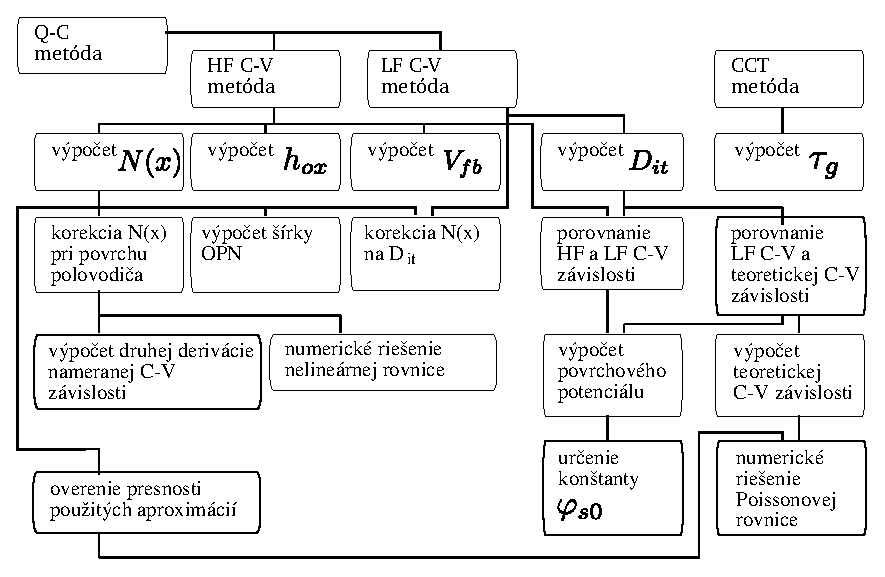
\includegraphics[width=\textwidth,height=\textheight,scale=0.7,keepaspectratio]{Figures/diagram-1.EPS}\label{diagram:1}
\end{diagram}

\section{High frequency C-V method.}\label{sec:3.1}

In the high-frequency capacitance method measurement, the MOS structure
is brought to the desired state by a DC gate voltage and its
capacitance is determined from the current response to a
high-frequency signal of small amplitude, which is superimposed on the
DC gate voltage. By measuring the phase shift between the
high-frequency voltage signal and current, in addition to the
capacitance, it is also possible to evaluate the conductivity of the
structure. The magnitude of the frequency of the measurement signal is
determined by the trade-off between the requirement of the highest
possible frequency from the influence measurement by the fast traps of
the $Si-SiO_2$ interface and the technical possibilities of standard
measuring instruments.  In our experiment we used the HP4280a
instrument, whose measurement signal has a fixed frequency 1 MHz and
the amplitude of the measurement signal can be selected as 10 mV, or
30 mV.  The above mentioned instrument can be controlled using the
GPIB bus. It should be It should be noted that the instrument, in
conjunction with the PC AT control system, is capable of block
transfer to measure and transfer in binary format to the control 680
points (which is the limit for block transfer) of C-V and G-V
dependencies in 25 seconds.  The above time figure is based on our own
experiments.

\section{Quasi-static C-V method.}\label{sec:3.2}

In the quasi-static capacitance method measurement, the MOS structure
is charged by a slow, increasing gate voltage over time. The
capacitance of the MOS structure is determined as a function of the
charging current and the rate of rise of the gate voltage.  Hence, to
implement the method, it is a source of continuously increasing
voltage is required and ammeter. The rate of voltage rise must be
small enough to the structure is still in thermodynamic equilibrium
during the measurement. At On the other hand, as the rate decreases,
the current which we have to measure. For most of the samples
measured, a velocity of the order of $10^{-2}V/s$, which for a
capacitance of $100pF$ represents the charging current $10^{-12}A$. In
our experiment, we used a charge-current Keithley 642 electrometer,
which measures current in the range of $10^{-8}A$ to $10^{-17}A$ with
a resolution of 5 digits per range.  It should be noted that in
addition to the other excellent features of the instrument, the
manufacturer guarantees an effective noise figure of less than
$8\times10^{-17}A$. The source of the increasing voltage, which was
built in our department, allows the adjustment of the rate of voltage
rise in the range from $10V/s$ to $10^{-3}V/s$ with with a resolution
of 1\% of the range. Both devices can be controlled using the bus
GPIB.  The main source of error in the quasi-static method is the
inaccuracy of the determination of the gate voltage rise
rate~\cite{1.5}. Before each measurement, it is necessary to
accurately measure the rate of voltage rise, which is then used in the
capacitance calculation. The rate of voltage rise for selected range
is determined in our case from the ratio of the voltage change and the
time in 10 s. This value then has the meaning of a mean value and its
use in the calculation assumes a linear increase in voltage, which we
experimentally verified for a representative sample of voltage rise
ranges of voltage over time.

\section{Q-C method.}\label{sec:3.3}

Q-C method\cite{3.4} is a combination of high frequency C-V method and
the charge Q-V method~\cite{3.5}. Its principle is is as follows. In
series with a condenser formed by a MOS structure, the
voltage-independent capacitance, which we denote by $C_i$.  At
series-parallel connection of the capacitors, which is shown in
Figure~\ref{fig:3.1}, we connect a DC voltage $V_a$ and measure the
voltage $V_i$ at the common point of the capacitor connections, which
represent capacitive divider. The capacitors labeled $C_w$ and $C_x$
show parasitic capacitances. $C_w$ is the capacitance between the
table and the raised probe tip and $C_x$ is the capacitance of the
common point of connection of the capacitors with respect to
ground. At the same time as measuring the voltage $V_i$, we also
measure capacitance $C_m$ and conductivity $G_m$ using a high
frequency signal superimposed on the voltage $V_a$.

\begin{figure}[h!]\centering
  \includegraphics{Figures/fig-3-1.eps}% chktex-file 8
  \caption[Schematic illustration of Q-C capacitor wiring
    methods]{Schematic representation of Q-C capacitors wiring
    methods}\label{fig:3.1}
\end{figure}

Between the common point of the capacitor wiring and the voltmeter
input is a resistor is connected which, together with the capacitance
of the voltmeter lead wires and the input capacitance of the voltmeter
form a low-pass filter, causing the measured voltage to be unaffected
by high-frequency signal. It also follows that the magnitude of the
capacitance between the common point of connection and point L will be
different for DC and high-frequency measurements. Let us therefore
denote the capacitance $C_i$ for DC measurement $C_{iLF}$ and for high
frequency measurement $C_{iHF}$.  Mentioned resistance together with
the input resistance of the voltmeter forms the voltage divider.  To
the voltage measurement is not affected, a voltmeter with high input
resistance.  The suitability of using the Keithley 642 meter, whose
input resistance in the measurement mode is approximately $10^{16}
\Omega$ and its parasitic input capacitance is $2 pF$. A detailed
description of the circuit of the Q-C method, eliminating of parasitic
capacitances, or the methodology of their measurement, is described in
Appendix~\ref{app:AppendixE}. If we know the capacitance of the oxide
layer of the MOS structure $C_{ox}$ and the magnitude of the
capacitance $C_{iLF}$, we can calculate the value of the surface
potential $\varphi_s$ from the following relation, derived in
Appendix~\ref{app:AppendixF}.

\begin{equation}\label{eq:3.1}
  \varphi_s = \varphi_{s0} + V_g (1 + \frac{C_w}{C_{ox}}) - V_i \frac{C_{iLF}+C_x}{C_{ox}}
\end{equation}

At the same time, we can determine the low-frequency capacitance of
the MOS structure

\begin{equation}\label{eq:3.2}
  C^{LF}_{mos} = C_{ox} (1 - \frac{d\varphi_s}{dV_g})
\end{equation}

The defect charges present in the measured MOS structure cause the
surface potential of the semiconductor assumes the value
$\varphi_{s0}$ even at zero gate voltage. The magnitude of this
constant can be determined from a comparison of the measured and
theoretical dependence of the surface potential on the SCR width
$\varphi(x)$.  The method for determining $\varphi_{s0}$ is described
in Appendix~\ref{app:AppendixG}. It may be noted here that to
calculate $C^{LF}_{mos}$ the value of this constant is not needed, as
can be seen from equations~\ref{eq:3.1} and~\ref{eq:3.2}.

From the measured values of $C_m$ and $G_m$ we can determine the high
frequency capacitance of the MOS structure using the following
relations.  First calculate the corresponding resistance $R_m$ and
reactance $X_m$

\begin{subequations}\label{eq:3.3}
  \begin{align}
    R_m &= \frac{G_m}{G^2_m + {(\omega C_m)}^2}\label{eq:3.3a}\\[0.3cm]
    X_m &= \frac{\omega C_m}{G^2_m + {(\omega C_m)}^2}\label{eq:3.3b}\\[0.3cm]
    \intertext{,which we use in the relation}
    C^{HF}_{mos} &= - \cfrac{R^2_m + {(X_m + \frac{1}{\omega C_{iHF}} + \omega C_w D^2)}^2}{\omega D^2{(X_m + \frac{1}{\omega C_{iHF}} + \omega C_{w} D^2)}^2}\label{eq:3.3c}\\[0.3cm]
    \intertext{,where}
    D^2 &= R^2_m + {(X_m + \frac{1}{\omega C_{iHF}})}^2\label{eq:3.3d}
  \end{align}
\end{subequations}

A detailed description and derivation of the above relationships is
described in the Appendix~\ref{app:AppendixE}. The Q-C method provides
a number of advantages.  It allows simultaneous measurement of high
and low frequency C-V dependence, guaranteeing the same measurement
conditions for both dependencies, and eliminates the possibility of
their mutual voltage drift, which can occur if the dependencies were
sensed sequentially.  At the same time, the measurement of the
low-frequency C-V dependence is static and does not depend on the
dynamics of the gate voltage.

To determine the concentration profile of impurities in the subsurface
of the semiconductor, it is advantageous to know the surface potential
curve, which allows calculation unencumbered by the traps of the
$Si-SiO_2$ interface. Cited by advantages are offset by the difficulty
of the method for the instrumentation used.  A critical point in the
implementation of the method is the stripping of the common point of
the capacitors. The connected voltage $V_a$ must be decomposed into
capacitors according to their capacitances and not according to their
leakage resistances.  This requires the use of a good quality
capacitor $C_i$ and the arrangement of of the individual components of
the method so that the leakage current from a common point to ground
is as small as possible. This makes the use of the Q-C method excludes
MOS structures that have large leakage currents due to imperfections
in the oxide layer. For measurements in the thermodynamic state
equilibrium, as stated by the authors of the method~\cite{3.7}, it is
necessary to the voltage $V_i$ to remain unchanged for at least 10
seconds by an order of magnitude $10^{-3}V$. For the purpose of
determining the concentration profile, we can measure non-equilibrium
C-V dependence, where the leakage currents from the common point to
ground do not manifest themselves to such an extent because the
measured voltage is read immediately after the voltage is applied. In
Figure~\ref{fig:3.2} the shows the normalized curves of the HF C-V
dependence of the MOS structure and surface potential curves with
respect to the gate voltage determined by Q-C method for measurements
in the thermodynamic equilibrium state and in the deep depletion. The
instruments used in the implementation of the method on our
department~\cite{3.8,3.9} can be controlled using the GPIB bus and
the measured values of voltages $V_a$, $V_i$, capacitance $C_m$ and
conductivity $G_m$ can be stored in a disk file for further
processing.

\begin{figure}[h!]\centering
\includegraphics{Figures/fig-3-2.eps}
\caption[Normalized curves HF C-V dependence of MOS structure and curve
  surface potential versus gate voltage determined using the Q-C method
  for measurements in thermodynamic equilibrium and deep
  depletion]{Normalized HF C-V curves of the structure
  MOS and surface potential curves from gate voltage determined
  using the Q-C method for measurements in the thermodynamic equilibrium state and in
  deep depletion state. The $\varphi_s(V_g)$ curves are shown
  using the normalization $1-\frac{\varphi_s}{\varphi_{norm}}$, where
  $\varphi_{norm}=3.33V$.}\label{fig:3.2}
\end{figure}
%OBR7.BIT

To verify the accuracy of the Q-C method, we have used the same MOS
structure we performed separate high and low frequency measurements
and simultaneously calculated the same capacitance dependencies from
the measured values Q-C method.  The resulting curves are shown in
Figures~\ref{fig:3.3} and~\ref{fig:3.4}.

For a quantitative comparison of the results shown in
Fig.~\ref{fig:3.3} and~\ref{fig:3.4}, we present in
Table~\ref{tab:3.1} and~\ref{tab:3.2} numerical values of the
normalized capacitances $C^{HF}_{mos}$ and $C^{LF}_{mos}$ for the HF,
LF and Q-C methods and their difference in terms of relative
error. The tables show the difference between the C-V dependencies,
which is due both to inaccuracies in the determination of of the
parasitic capacitances and secondly the leakage currents used
capacitors. The authors of the method recommend to eliminate leakage
of leakage currents caused by the humidity of the environment, use an
air capacitor $C_i$ and to direct a current to the sample to be
measured during the measurement to prevent condensation of water
vapour from the surroundings.

\newpage
\begin{figure}[h!]\centering
  \includegraphics{Figures/fig-3-3.eps}
  \caption[Normalized capacitance curves of MOS structure with substrate type
  N as a function of gate voltage for equilibrium high-frequency and
  quasi-static measurements]{Normalized capacitance curves of a MOS structure with
  N-type substrate as a function of gate voltage for equilibrium
  high-frequency and quasi-static measurements.  At the same time, those
  same characteristics obtained by the Q-C method. For completeness, the
  the dependence of the surface potential
  ${\varphi_s(V_g)}^{QC}$ obtained using the Q-C method and the dependence
  ${\varphi_s(V_g)}^{LF}$ calculated by integrating the low-frequency C-V
  dependence using the Berglund integral.  Flows
  $\varphi_s(V_g)$ are shown using the normalization $1-\frac{\varphi_s}{\varphi_{norm}}$, where $\varphi_{norm}=-3.33V$.}\label{fig:3.3}
\end{figure}
%OBR5.BIT

\begin{table}[h!]\centering
  \begin{tabular}{c c c c c c}
    \multicolumn{3}{l}{$C^{HF}_{mos}$} & \multicolumn{3}{l}{$C^{LF}_{mos}$} \\
    HF[\%] & QC[\%] & $\Delta_r$[\%] & LF[\%] & QC[\%] & $\Delta_r$[\%] \\
    \hline% chktex-file 44
    99.67 & 98.30 & +1.37 & 97.85 & 99.14 & -1.32 \\
    98.56 & 96.69 & +1.89 & 96.59 & 97.05 & -0.47 \\
    98.56 & 96.69 & +1.89 & 96.59 & 97.05 & -0.47 \\
    95.73 & 93.89 & +1.92 & 93.93 & 94.51 & -0.61 \\
    89.89 & 87.75 & +2.39 & 88.26 & 88.57 & -0.36 \\
    82.15 & 80.17 & +2.41 & 81.43 & 81.82 & -0.47 \\
    74.83 & 73.09 & +2.33 & 73.79 & 74.57 & -1.06 \\
    69.69 & 67.81 & +2.70 & 86.08 & 86.33 & -0.29 \\
    69.10 & 67.20 & +2.74 & 97.20 & 97.73 & -0.54 \\
    68.97 & 67.08 & +2.74 & 98.27 & 98.74 & -0.48 \\
    68.91 & 67.03 & +2.72 & 98.75 & 99.38 & -0.64 \\
    68.90 & 67.01 & +2.75 & 99.04 & 98.68 & -0.36 \\
    68.90 & 67.03 & +2.70 & 99.20 & 99.87 & -0.67 \\
  \end{tabular}
  \caption[Comparison of normalized frequency and low-frequency
    capacitance of the MOS structure (Figure~\ref{fig:3.3}) for HF, LF
    and Q-C methods]{Comparison of normalized high-frequency and
    low-frequency capacitance of the MOS structure
    (Figure~\ref{fig:3.3}) for HF, LF and Q-C methods. The difference
    of the curves is expressed by the relative error.}\label{tab:3.1}
\end{table}

\newpage
\begin{figure}[h!]\centering
%\framebox[10cm]{\rule{0cm}{3cm}}
\includegraphics{Figures/fig-3-4.eps}
\captionsetup{justification=raggedright, singlelinecheck=false}
\caption[Normalized capacitance curves of MOS structure with substrate type
  P as a function of gate voltage for equilibrium high-frequency and
  quasi-static measurements]{Normalized capacitance curves of a MOS structure with
  P-type substrate as a function of gate voltage for equilibrium
  high-frequency and quasi-static measurements.  At the same time, those
  same characteristics obtained using the Q-C method. For completeness, the
  the dependence of the surface potential
  ${\varphi_s(V_g)}^{QC}$ obtained using the Q-C method and the dependence
  ${\varphi_s(V_g)}^{LF}$ calculated by integrating the low-frequency C-V
  dependence using the Berglund integral. Flows
  $\varphi_s(V_g)$ are shown using the normalization $1 -
  \frac{\varphi_s}{\varphi_{norm}}$, where $\varphi_{norm}=3.33V$.}\label{fig:3.4}
\end{figure}
%OBR6.BIT

\begin{table}[h!]\centering
  \begin{tabular}{c c c c c c}
    \multicolumn{3}{l}{$C^{HF}_{mos}$} & \multicolumn{3}{l}{$C^{LF}_{mos}$} \\
    HF[\%] & QC[\%] & $\Delta_r$[\%] & LF[\%] & QC[\%] & $\Delta_r$[\%] \\
    \hline
    96.30 & 95.71 & +0.62 & 94.80 & 94.89 & -0.09 \\
    92.88 & 92.07 & +0.87 & 91.03 & 92.83 & -1.98 \\
    87.52 & 86.48 & +1.19 & 85.97 & 87.53 & -1.81 \\
    81.39 & 80.09 & +1.60 & 79.70 & 81.20 & -1.88 \\
    75.71 & 74.55 & +1.53 & 74.24 & 76.00 & -2.37 \\
    71.17 & 69.79 & +1.98 & 69.89 & 70.65 & -1.08 \\
    67.77 & 66.41 & +2.00 & 80.77 & 83.57 & -3.47 \\
    67.14 & 65.85 & +1.93 & 94.72 & 96.93 & -2.33 \\
    66.82 & 65.73 & +1.62 & 96.77 & 98.26 & -1.53 \\
    66.65 & 65.63 & +1.52 & 97.47 & 98.06 & -0.60 \\
    66.62 & 65.59 & +1.53 & 97.94 & 99.46 & -1.56 \\
    66.58 & 65.54 & +1.56 & 98.15 & 99.39 & -1.26 \\
  \end{tabular}
  \caption[Comparison of normalized frequency and low-frequency
    capacitance of the MOS structure (Figure~\ref{fig:3.4}) for HF, LF
    and Q-C methods]{Comparison of normalized high-frequency and
    low-frequency capacitance of the MOS structure
    (Figure~\ref{fig:3.4}) for HF, LF and Q-C methods. The difference
    of the curves is expressed by the relative error.}\label{tab:3.2}
\end{table}

\section{Constant-width SCR method and determination of the generation lifetime of minority charge carriers.}\label{sec:3.4}

The substrate quality of the MOS slit can be judged from the
generation time lifetime of the minority charge carriers, which we
will denote by $\tau_g$. The classical method of determining this
parameter is the Zerbst method~\cite{3.2}, which determines $\tau_g$
from the relaxation transition time of the MOS structure from the
non-equilibrium state to the equilibrium state. Currently the
semiconductor industry is working with high quality silicon wafers,
whose relaxation times are in the order of tens of minutes, which
precludes the effective use of the Zerbst method in controlling
semiconductor technology. Significant acceleration of the
determination process $\tau_g$ of high quality silicon substrates is
made possible by the constant width SCR~\cite{3.1}. Its principle is
as follows. The MOS structure is brought to a non-equilibrium state by
a voltage pulse at the gate of deep depletion. The generation of
minority charge carriers causes the formation of an inversion layer on
the semiconductor surface, shading the substrate and subsequent SCR
tapering, which is manifested by an increase in the capacitance of the
structure MOS\@. The effect of the generation of minority charge
carriers on the width of the SCR can be be compensated by increasing
the gate voltage and thus ensuring a constant width of the
SCR\@. Obviously, the rate of increase of the gate voltage will depend
on the rate of generation of minority charge carriers, which can be
expressed by the following equation~\cite{3.3}

\begin{equation}\label{eq:3.4}
  I_g = C_{ox} \frac{dV_g}{dt}
\end{equation}

where $I_g$ represents the generation current of minority charge carriers that
form the inverse layer.  The generational lifetime of the minority carriers
$\tau_g$ can then be expressed using the generation current $I_g$~\cite{3.3}

\begin{equation}\label{eq:3.5}
  \tau_g = \frac{qxn_i}{2I_g}
\end{equation}

In the above method, we assume that the charge increment in the
inverse layer is made up only of minority charge carriers that are
generated in the SCR\@. This neglects the diffusion of minority
carriers from the substrate and the surface of the semiconductor,
which may distort the measured results. Distortion results can occur
especially if the space in which the the measured sample is not
perfectly sealed, which causes ingress light in. The electron-hole
pairs generated by the photons trapped on the the surface of the
semiconductor, contribute to the generation current and the calculated
values of $\tau_g$ will be less than their actual value.  Impact of
the above phenomena can be eliminated if we determine $\tau_g$ from
the difference of the measured $V_g(t)$ dependence directions for
different widths SCR~\cite{3.3, 3.10, 3.11, 3.12}. The generation
current, formed by the minor charge carriers that are generated in the
SCR, can then be expressed by the relation

\begin{equation}\label{eq:3.6}
  I_g = C_{ox} \bigg[\frac{dV_g}{dt}\Big\rvert_{C_1} - \frac{dV_g}{dt}\Big\rvert_{C_2}\bigg]
\end{equation}

and the generation time $\tau_g$

\begin{equation}\label{eq:3.7}
  \tau_g = \frac{q\Delta x n_i}{2I_g}
\end{equation}

where $\Delta x$ is the distance by which the SCR is expanded when the
capacity changes from $C_1$ to $C_2$

\begin{equation}\label{eq:3.8}
  \Delta x = \epsilon \Big[\frac{1}{C_2} - \frac{1}{C_1}\Big]
\end{equation}

The calculated value of $\tau_g$ from the equation~\ref{eq:3.7} is
then the mean value of the generational lifetime of the minority
charge carriers in the region of the semiconductor defined by the
distance $\Delta x$.  Issues of non-equilibrium measurements has been
treated in our department in paper~\cite{1.6} and an analog
implementation of the above method has been has been treated in
Thesis~\cite{3.13}. Part of this dissertation is A numerical
implementation of the constant-width method SCR\@. In order to measure
capacitance was used to measure the HP4280a instrument, which also
contains a source of DC voltage source. The method was automated using
a bus GPIB. The most important part of the control program is the
loop, in which maintains the constant capacitance of the MOS structure
in non-equilibrium state by varying the gate voltage.  If we know the
curve concentration profile in the semiconductor, we can calculate
the necessary change gate voltage for a measured change in the
capacitance of the MOS structure from equation~\ref{eq:3.3}

\begin{equation}\label{eq:3.9}
  \frac{dV_g}{dC_{mos}} = \frac{q\epsilon N}{C^3_{mos}}
\end{equation}

If we measure time at the same time, we get the dependence
$V_g(t)$. Measurement procedure one dependence $V_g(t)$ is shown by
the following evolution diagram.

\begin{diagram}
  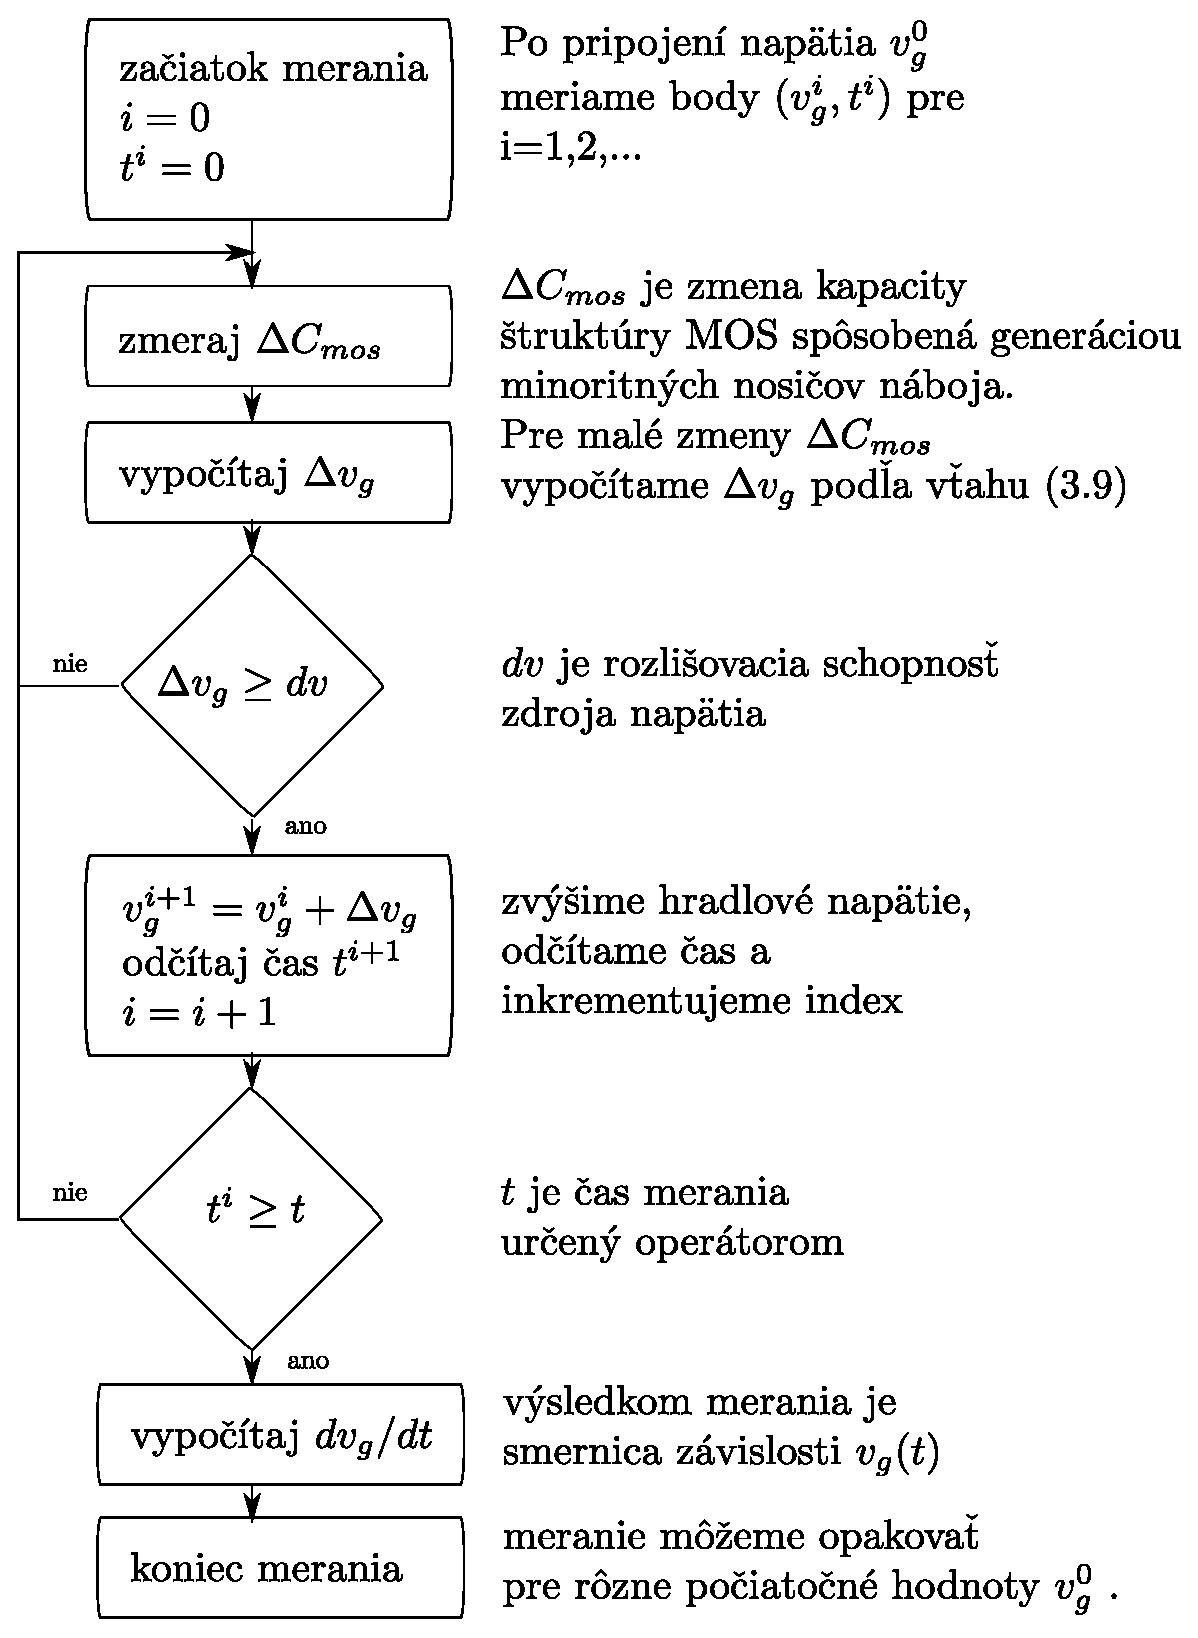
\includegraphics[scale=0.55,keepaspectratio]{Figures/diagram-2.EPS}\label{diagram:2}
\end{diagram}

\begin{figure}[h!]\centering
  \includegraphics{Figures/fig-3-5.eps}
  \caption[Dependence of $\frac{dV_g}{dt}$ on SCR width obtained by
    constant SCR width method]{Dependence of $\frac{dV_g}{dt}$ on width
    SCR obtained using the constant width SCR method.}\label{fig:3.5}
\end{figure}
%OBR19.BIT

Figure~\ref{fig:3.5} shows the dependence of $\frac{dV_g}{dt}$ on
of the width of SCR\@. Assuming the SCR width is kept constant, the
potential ratios in the semiconductor and the generation of minority carriers is
constant, implying a linear dependence of $V_g(t)$.  Guidelines
${frac{dV_g}{dt}}$ can then be determined by linear regression of the measured
$V_g(t)$ dependence. It is not difficult to imagine that
equations~\ref{eq:3.6} to~\ref{eq:3.8} represent the discrimination
of the continuous curve $\tau_g(x)$. If the measured values
$\frac{dV_g}{dt}=f(x)$ are approximated by a continuous function, we can express
the depth profile $\tau_g(x)$ by the relation

\begin{equation}\label{eq:3.10}
  \tau_g(x) = \frac{qn_i}{2C_{ox}} {\Bigg[\frac{d\big[\frac{dV_g}{dt}\big]}{dx}\Bigg]}^{-1}
\end{equation}

Figure~\ref{fig:3.6} shows the curve of $\tau_g(x)$, calculated
from the measured data shown in Figure~\ref{fig:3.5} and in
Figure~\ref{fig:3.7} is the depth concentration profile $N(x)$ of the investigated
structure.

\begin{figure}[h!]\centering
  \includegraphics{Figures/fig-3-6.eps}
  \caption[Depth profile of the generation lifetime of minority carriers
    charge]{Depth profile of the generation time of minority carriers
    of the minority of the charge.}\label{fig:3.6}
\end{figure}
%OBR20.BIT

\begin{figure}[h!]\centering
  \includegraphics{Figures/fig-3-7.eps}
  \caption[Depth profile of concentration of interfering impurities
    $N(x)$]{Depth concentration profile of interfering impurities
    $N(x)$. The impurity concentration profile was created by implanting
    $P^{31}$ with a dose of $8.0$ $10^{15}m^{-2}$ at an energy of $120 keV$.
    The activation was carried out for 40 minutes at a temperature of $1050 \degree C$ in
    $N_2$ atmosphere.}\label{fig:3.7}
\end{figure}
%OBR21.BIT


\begin{thebibliography}{}

\bibitem[3.1]{3.1}
  Pierret R.F., Small D.W.: IEEE Trans.\ on elektron.dev. 22 (1975) s.1052.

\bibitem[3.2]{3.2}
  Zerbst M.. Angew. Phys. 22 (1966), p.30.

\bibitem[3.3]{3.3}
  Eades W.D., Shott J.D., Swanson R.M.: IEEE Trans.\ on elektron.\ dev. 30 (1983) s.1274.

\bibitem[3.4]{3.4}
  Nicollian E.H., Brews J.R.: Solid St.\ Electron.  27 (1984) s.953.

\bibitem[3.5]{3.5}
  Ziegler K., Klausmann E.: Appl. Phys. Leta. 26 (1975) p.400.

\bibitem[3.6]{3.6}
  Boulin D.M., Brews J.R., Nicollian E.H.: Solid St.\ Electron. 27 (1984) s.977.

\bibitem[3.7]{3.7}
  Brews J.R., Nicollian E.H.: Solid St.\ Electron. 27 (1984) s.963.

\bibitem[3.8]{3.8}
  Botka V.,Csabay O., Jamrich M.: 5th national conference Microelectronics 1989, House of Technology CSVTS Bratislava, 1989 p.59.

\bibitem[3.9]{3.9}
  Jamrich M.: Q-C method for the investigation of MIS\@ structures. Diploma thesis, Department of Microelectronics, EF SVŠT, Bratislava 1988.

\bibitem[3.10]{3.10}
  Beyer A., Markgraf W.: Wiss. Z. d. Techn. Hochsch. Karl-Marx-Stadt 28 (1986) p.479.

\bibitem[3.11]{3.11}
  Lal, Vasi: Solid St.\ Electron. 30 (1987) s.801.

\bibitem[3.12]{3.12}
  Hof, Morthers, Roenker: Solid St.\ Electron. 31 (1988) s.937.

\bibitem[3.13]{3.13}
  Pilka K.: Non-equilibrium capacitive method with constant width SCR, Department of Microelectronics, EF SVŠT, Bratislava 1989.

\end{thebibliography}

% Chapter 4

\chapter{Methods for determination of other parameters of MOS structure.}\label{Chapter4}
\lhead{Chapter 4. \emph{Methods for determination of other parameters of MOS structure}}
%- - - - - - - - - - - - - - - - - - - - - - - - - - - - - - - - - - - - - - - - - - - -

In Chapter~\ref{Chapter3} we have described the C-V methods that we
will use to determine the parameters of MOS\@ structures. In
particular, we we will deal with the determination of the
concentration profile of the donating impurities in the subsurface
region of the semiconductor, since some methods of determining other
MOS structure parameters are based on the assumption that the
concentration is known. In determining the concentration profile
curves, which are not homogeneous, models are used whose accuracy
of approximating a given physical phenomenon depends on the
concentration gradient admixture~\cite{4.1, 4.2, 4.3, 4.4}. In order
to verify the accuracy of the used approximations, we performed a
comparison of the concentration profiles:

\begin{itemize}
\item used in the calculation of the theoretical C-V dependence and
\item obtained from this theoretical C-V dependence~\cite{4.5}.
\end{itemize}

The results are given in Section~\ref{sec:4.1.4}.

\par The next parameter we will determine is the density of traps
of the $Si-SiO_{2}$ interface. Here, two
procedures. Comparison of high and low frequency C-V
dependence, or a comparison of experimental and theoretical C-V
dependence. Their application is described in Section~\ref{sec:4.2}.

\par Determination of the generation lifetime of minority charge carriers that
related to the constant-width SCR method, has been described in Section~\ref{sec:3.4}.

\section[Determination of the concentration profile of impurities]{Determination of the concentration profile of impurities in the subsurface region of the semiconductor.}\label{sec:4.1}

The subject of measuring concentration profiles was addressed in our
department in the paper~\cite{4.6}. Here we will address only some
aspects of this subject that are related to the determination of
inhomogeneous concentration profile of dopants in a semiconductor.

\par Separate areas of concern in determining the concentration
profile of impurities, which we denote by $N(x)$, consist of:

\begin{itemize}
\item correction of the calculated concentration in the region from
  the surface of the semiconductor to a depth of $2L_{DE}$~\cite{4.7,
    4.8}
\item determination of the depth of the calculated concentration,
  relying on models determining the width of the SCR~\cite{4.9, 4.10,
    4.11}
\item correction for the effect of $Si-SiO_2$ interface
  traps~\cite{4.12}
\item the difference between the concentration of the interfering
  impurities $N(x)$ and the concentration of the majority charge
  carriers $n(x)$.
\end{itemize}

\subsection[Correction of the concentration of interfering impurities]{Correction of the concentration of interfering impurities at the surface of the semiconductor.}\label{sec:4.1.1}

Known equation for calculating $N(x)$~\cite{I.2}

\begin{equation}\label{eq:4.1}
  N(x) = {\frac{2}{q\epsilon}} {\Bigg[\frac{dC_{sc}^{-2}}{d\varphi_{s}}\Bigg]}^{-1}
\end{equation}

was derived from the solution of the Poisson equation using the
approximation of deep depletion. This approximation does not hold for
SCR widths smaller than $2L_{DE}$. In order to obtain correct results
also in this region, we need to correct $N(x)$ computed according
to~\ref{eq:4.1} by the procedure derived in~\cite{4.7, 4.8}.  The
correction is a function of the surface potential. Its physical
significance is evident from the work~\cite{4.7}.

\begin{equation}\label{eq:4.2}
  {N(x)}_{corrected} = N(x)f(\varphi_{s})
\end{equation}

, where

\begin{equation}\label{eq:4.3}
  f(\varphi_{s}) = {\frac{1}{1-e^{-\beta\varphi_{s}}}} - {\frac{2e^{-\beta\varphi_{s}}\big[e^{-\beta\varphi_{s}}+\beta\varphi_{s} -1\big]}{\big[1-e^{-\beta\varphi_{s}}\big]}} \qquad, where\quad \beta=\frac{q}{kT}
\end{equation}

The surface potential used in equation~\ref{eq:4.3} can be determined
according to~\cite{4.7} by numerically solving the equation

\begin{equation}\label{eq:4.4}
  \frac{C_{sc}^{2}}{\varphi_{s}}\frac{C_{sc}^{-2}}{d\varphi_{s}}=\frac{1-e^{-\beta\varphi_{s}}}{e^{-\beta\varphi_{s}}+\beta\varphi_{s}-1}-\frac{2e^{-\beta\varphi_{s}}} {1-e^{-\beta\varphi_{s}}}
\end{equation}

It should be noted here that the equation~\ref{eq:4.4} was derived
using the relation for the SCR capacity $C_{sc}$, which assumes a
homogeneous concentration of dopants. Since the experimentally
determined differential capacitance $C_{sc}$ depends on the change in
charge at the SCR boundary (which uses equation~\ref{eq:4.1}), the
surface potential obtained from equation~\ref{eq:4.4} will represent
the potential that would be at the surface of the semiconductor if the
concentration of $N(x)$ across the SCR region were constant and also
equal to the concentration at the SCR boundary (which we determine
according to~\ref{eq:4.1}). It follows that for inhomogeneously doped
substrates the equation~\ref{eq:4.4} cannot be used to obtain the true
values of $\varphi_{s}(V_{g})$, despite the fact that the
correction~\ref{eq:4.2} gives good results in this case as well.

\subsection[Determination of the depth of the concentration profile.]{Determination of the depth of the concentration profile.}\label{sec:4.1.2}

Having determined the concentration according to the
equation~\ref{eq:4.2}, it is also necessary to determine the location
of the calculated concentration. A commonly used relationship based on
plate capacitor model (which is an approximation of the deep
depletion)

\begin{equation}\label{eq:4.5}
  w(C_{sc})=\frac{\epsilon}{C_{sc}}
\end{equation}

is not valid for depths less than $2L_{DE}$. In this region, it is
possible to use the relation derived using an approximation of the
curve of the electric potential in semiconductor $\varphi(x)$. The
above problem has been discussed in detail in our department
in~\cite{4.13, 4.14}, where the results of work~\cite{4.9, 4.10, 4.11}
were used. To calculate the depth in this region, we can use a
relation that is an approximation of the curve of the electric
potential in semiconductor $\varphi(x)$~\cite{I.1}

\begin{equation}\label{eq:4.6}
  w(\varphi_{s})=\sqrt{2}L_{DE}{\big[e^{-\beta\varphi_{s}}+\beta\varphi_{s}-1\big]}^{\frac{1}{2}}
\end{equation}

, where

\begin{equation}\label{eq:4.7}
  L_{DE} = {\Big[\frac{\epsilon}{\beta qN}\Big]}^{\frac{1}{2}}
\end{equation}

is the extrinsic Debay length, which we used in the calculation the
concentration obtained from the equation~\ref{eq:4.2}.  In
equation~\ref{eq:4.6} we use the value of $\varphi_{s}$ obtained from
the solution equation~\ref{eq:4.4}. Despite the fact that also the
equation~\ref{eq:4.6} was derived assuming a homogeneous distribution
of impurities in the semiconductor, its use in conjunction with the
solution of equation~\ref{eq:4.4} gives a satisfactory results, as we
shall show later.

\begin{figure}[h!]\centering
  \begin{minipage}[c]{\myfiguresize}
    \begin{center}
      \includegraphics{Figures/fig-4-1.eps}% chktex-file 8
      \caption[Concentration profile of dopants in a semiconductor
        calculated from the equation~\ref{eq:4.2}]{Concentration
        profile of the dopants in the semiconductor calculated from
        the equation~\ref{eq:4.2}. The distance from the surface was
        determined from the equation~\ref{eq:4.5} (curve 1)
        and~\ref{eq:4.6} (curve 2).}\label{fig:4.1}
    \end{center}
  \end{minipage}
\end{figure}
% OBR26.BIT

Figure~\ref{fig:4.1} shows the curves of $N(x)$ using
correction~\ref{eq:4.2}, presenting the difference in using
equations~\ref{eq:4.5} and~\ref{eq:4.6}. Here it is clear that by
using equation~\ref{eq:4.6} one can calculate the path of the
concentration of the dopants closer to the semiconductor surface.
This is of importance for further calculations, which presuppose
knowledge of the $N(x)$ curve.

The first column of the table~\ref{tab:4.1} contains the values of
$\varphi_{s}$ determined by solving the equation~\ref{eq:4.4} and the
second column contains the values of the correction
factor~\ref{eq:4.3}. The other two columns allow comparison of the
uncorrected and corrected values of $N(x)$ and the last two columns
give the values of $w(\varphi_{s})$ and $w(C_{sc})$ obtained from the
equations~\ref{eq:4.5} and~\ref{eq:4.6}.

\begin{table}[h!]\centering
  \begin{minipage}[c]{\myfiguresize}
    \begin{center}
      \begin{tabular}{c c c c c c c c c c}
        $\varphi_{s}[V]$ & $f(\varphi_{s})$ & $N[m^{-3}]$ & $N_{cor.}[m^{-3}]$ & $w(\varphi_{s})[\mu m]$ & $w(C_{SC})[\mu m]$ \\
        \hline% chktex-file 44
        0.007 & 0.39 & $0.35\times10^{23}$ & $0.14\times10^{23}$ & 0.0102 & 0.0389 \\
        0.016 & 0.44 & $0.33\times10^{23}$ & $0.15\times10^{23}$ & 0.0190 & 0.0413 \\
        0.024 & 0.50 & $0.31\times10^{23}$ & $0.15\times10^{23}$ & 0.0265 & 0.0438 \\
        0.032 & 0.56 & $0.29\times10^{23}$ & $0.16\times10^{23}$ & 0.0333 & 0.0466 \\
        0.041 & 0.61 & $0.28\times10^{23}$ & $0.17\times10^{23}$ & 0.0391 & 0.0494 \\
        0.049 & 0.66 & $0.27\times10^{23}$ & $0.18\times10^{23}$ & 0.0444 & 0.0523 \\
        0.057 & 0.71 & $0.26\times10^{23}$ & $0.18\times10^{23}$ & 0.0493 & 0.0553 \\
        0.065 & 0.76 & $0.25\times10^{23}$ & $0.19\times10^{23}$ & 0.0538 & 0.0585 \\
        0.073 & 0.80 & $0.24\times10^{23}$ & $0.19\times10^{23}$ & 0.0581 & 0.0617 \\
        0.081 & 0.83 & $0.23\times10^{23}$ & $0.19\times10^{23}$ & 0.0623 & 0.0650 \\
        0.090 & 0.86 & $0.22\times10^{23}$ & $0.19\times10^{23}$ & 0.0664 & 0.0684 \\
        0.098 & 0.89 & $0.22\times10^{23}$ & $0.19\times10^{23}$ & 0.0704 & 0.0719 \\
        0.106 & 0.91 & $0.21\times10^{23}$ & $0.19\times10^{23}$ & 0.0743 & 0.0755 \\
        0.115 & 0.93 & $0.21\times10^{23}$ & $0.19\times10^{23}$ & 0.0783 & 0.0791 \\
        0.124 & 0.94 & $0.20\times10^{23}$ & $0.19\times10^{23}$ & 0.0822 & 0.0828 \\
        0.133 & 0.96 & $0.20\times10^{23}$ & $0.19\times10^{23}$ & 0.0861 & 0.0866 \\
        0.142 & 0.97 & $0.19\times10^{23}$ & $0.19\times10^{23}$ & 0.0900 & 0.0904 \\
        0.151 & 0.97 & $0.19\times10^{23}$ & $0.18\times10^{23}$ & 0.0939 & 0.0942 \\
        0.160 & 0.98 & $0.19\times10^{23}$ & $0.18\times10^{23}$ & 0.0978 & 0.0981 \\
        0.169 & 0.99 & $0.18\times10^{23}$ & $0.18\times10^{23}$ & 0.1018 & 0.1019 \\
        0.178 & 0.99 & $0.18\times10^{23}$ & $0.18\times10^{23}$ & 0.1058 & 0.1058 \\
        0.187 & 0.99 & $0.18\times10^{23}$ & $0.17\times10^{23}$ & 0.1098 & 0.1098 \\
        0.205 & 1.00 & $0.17\times10^{23}$ & $0.17\times10^{23}$ & 0.1179 & 0.1179 \\
      \end{tabular}
      \caption[Calculation of dopant concentration profile
        $N(x)$]{Calculation of dopant concentration profile
        $N(x)$.}\label{tab:4.1}
    \end{center}
  \end{minipage}
\end{table}

\begin{minipage}[c]{\textwidth}
  \emph{NOTE.} Using the approximation~\ref{eq:4.6}, which represents
  the width of the SCR as as a function of the surface potential of
  the semiconductor (the concentration is parameter), one can
  approximate the path of $\varphi(x)$ for a given SCR width even if
  the semiconductor substrate is inhomogeneously doped.  Custom
  procedure for determining the concentration of dopant impurities
  from capacitance measurements is a discretization of the continuous
  $N(x)$ curve, where the individual values of $N_i$ represent an
  approximation of the concentration in the region of the boundary
  SCR~\cite{4.1, 4.2, 4.3}.  The loss of the potential
  $\Delta\varphi_i$ at layer of width $\Delta w_{i}=w_{i+1}-w_{i}$
  with concentration $N_i$ can be determined by solving the equation
  \begin{equation}\label{eq:4.8}
    \Delta w_{i} = \sqrt{2}L_{DE_{i}}{\Big[e^{-\beta\Delta\varphi_{i}} + \beta\Delta\varphi_{i} - 1\Big]}^{\frac{1}{2}}
  \end{equation}
  , where% chktex-file 26
  \begin{equation}\label{eq:4.9}
    L_{DE_{i}} = {\bigg[\frac{\epsilon}{\beta qN_{i}}\bigg]}^{\frac{1}{2}}
  \end{equation}
  Then the progression of $\varphi(x)$ can be obtained using the
  equations~\ref{eq:4.8} and~\ref{eq:4.9} if we start the calculation
  from the SCR boundary, where we assume potential is zero, towards
  the surface of the semiconductor.
\end{minipage}

\subsection[Effect of $Si-SiO_{2}$ interface traps and minority charge carrier generation]{Effect of $Si-SiO_{2}$ interface traps and minority charge carrier generation}\label{sec:4.1.3}

Minority carrier generation occurs in the inversion region of the SCR
charge generation, which forms the inversion layer and affects the
magnitude of the capacitance of the MOS\@ structure. In order to
measure the C-V dependence in the deep depletion that is not affected
by minority charge carriers, we will use the pulsed HF C-V method. The
measured values of $N(x)$ obtained using this method are shown in
Figure~\ref{fig:4.2}.

\begin{figure}[h!]\centering
  \begin{minipage}[c]{\myfiguresize}
    \begin{center}
      \includegraphics{Figures/fig-4-2.eps}% chktex-file 8
      \caption[Concentration profile of interfering impurities
        obtained from C-V dependence in the deep depletion region and
        from the equilibrium C-V dependence]{Current concentration
        profile of the interfering impurities obtained from the C-V
        dependence in the deep depletion region (curve 1) and from the
        equilibrium C-V dependence (curve 2). To calculate $N(x)$
        dependence, the C-V dependences shown in
        Figure~\ref{fig:3.2}}\label{fig:4.2}
    \end{center}
  \end{minipage}
\end{figure}
% OBR8.BIT

\par When calculating $N(x)$ using
equations~\ref{eq:4.1},~\ref{eq:4.2},~\ref{eq:4.3},~\ref{eq:4.4}
and~\ref{eq:4.6} the approximation is used

\begin{equation}\label{eq:4.10}
  \frac{dC_{sc}^{-2}}{d\varphi_{s}} \cong \frac{dC_{mos}^{-2}}{dV_{g}}
\end{equation}

where equality holds if the trap density of the $Si-SiO_{2}$ interface
is zero. However, the measured HF C-V dependence is always to some
extent affected by the interface traps, which change their
state~\cite{4.15}. This influence can be reduced by increasing the
frequency of the measurement signal and by measuring the capacitance
faster after the voltage jump pulsed C-V method.  The problem of using
the approximation~\ref{eq:4.10} is avoided if we use the data measured
by Q-C to determine $N(x)$ method, where we can determine the surface
potential curve $\varphi_{s}(V_{g})$. If we determine the
concentration profile of the dopants from the HF C-V dependence, we
can correct for the effect of the $Si-SiO_{2}$ interface traps in
depletion region by the relation given in~\cite{I.1}

\begin{equation}\label{eq:4.11}
  {N(x)}_{corrected} = {N(x)}{\cfrac{1-\cfrac{C_{mos}^{LF}}{C_{ox}}}{1-\cfrac{C_{mos}^{HF}}{C_{ox}}}}
\end{equation}

assuming we know the low-frequency C-V dependence.

\subsection[Calculation of the concentration profile of impurities from the curve of major charge carriers.]{Calculation of the concentration profile of impurities from the curve of major charge carriers.}\label{sec:4.1.4}

As can be seen from Figure~\ref{fig:1.1}, for the inhomogeneous
curve of the concentration of the donor atoms occurs due to
diffusion of the majority charge carriers, there is a difference
between the above curves~\cite{4.16}. It known~\cite{4.17} that by
using the equation~\ref{eq:4.1} we determine the curve of the
concentration of the majority charge carriers instead of the
concentration of the contaminating impurities. A correction is
described in the work of~\cite{4.18}, using the which can be used to
determine the exact concentration of the interfering atoms from the
measured $n (x)$ (if the measured $n (x)$ actually represents the
curve of the major charge carriers).

\begin{figure}[h!]\centering
  \begin{minipage}[c]{\myfiguresize}
    \begin{center}
      \includegraphics{Figures/fig-4-3.eps}
      \caption[Majority charge carrier concentration $n(x)$ determined
        from the depleted HF C-V dependence and the progression of the
        donating atoms $N (x)$ determined from the
        equation~\ref{eq:4.12}]{Concentration curve of major charge
        carriers $n (x)$ determined from the depleted HF C-V
        dependence and the path of the $N (x)$ donor atoms determined
        from equation~\ref{eq:4.12}.}\label{fig:4.3}
    \end{center}
  \end{minipage}
\end{figure}
% OBR23.BIT

\begin{equation}\label{eq:4.12}
  N(x) = n(x) - {\frac{kT\epsilon}{q^{2}} {\frac{d}{dx}} {\Bigg[\frac{1}{n(x)}\frac{dn(x)}{dx}\Bigg]}}
\end{equation}

Figure~\ref{fig:4.3} shows the curves of $n(x)$ and $N(x)$. In
equation~\ref{eq:4.12} the second derivative of $n(x)$ stands out,
which in the case of experimental values of $n(x)$ must be determined
numerically. Determining the derivative of an empirically obtained
functional dependence is a problem that can often be encountered when
processing measured data. In the basic numerical mathematics
courses~\cite{4.19} it is shown that differentiation amplifies the
noise of the processed data. In doing so, noise here generally refers
to the deviation of the processed data from its actual value that may
arise as a consequence of:

\begin{itemize}
\item physical phenomena
\item measurement instrument error
\item rounding in numerical processing.
\end{itemize}

\par That is, the frequency spectrum of the processed signal, obtained
by Fourier transformation, will contain components that must be
removed before (or during) the derivative calculation. V the following
we will talk about the approximation by polynomials, which most
commonly used, although the above statements also apply to other
classes of functions. If we use polynomial approximations to calculate
the derivative, the it is convenient to `smooth'~\cite{4.20} the
function values first. To suppress noise suppression, the frequency
properties of the numerical methods, which can be expressed in terms
of the transfer characteristics. This approach we can compare the
frequency properties of polynomial approximations and numerical
filters~\cite{4.21}.  The basic difference between the calculation of
the coefficients of digital filters and the coefficients of of
polynomial approximations is that in the first case we start from the
desired transmission characteristic and in the latter case are
coefficients are calculated from the least squares distance condition
of the processed data and the polynomial of a given degree. Hence
shortcomings of polynomial approximations:

\begin{itemize}
\item processed functional dependence may not be a polynomial, even
  though there is a polynomial that interpolates the measured values
\item frequency properties of the method are a secondary consequence
  of the degree of the polynomial used and the number of points
  through which the polynomial translates.
\end{itemize}

\par Because in our case we are processing functional dependencies
that are not polynomials in general, we have chosen to use numerical
filters. It may be mentioned here that for a successful application of
digital filters is important to design the critical frequency and
magnitude of the filter so that the filter does not affect the
amplitude of the signal in that part of the of the spectrum that
represents the useful signal. To determine the derivatives in
formula~\ref{eq:4.12}, we used a non-recursive differentiating
low-pass digital filter whose critical frequency is $f_{c}=0.1$ and
its size is $2n+1=11$.

\par It is known~\cite{4.18} that even the progression of $n(x)$,
determined from the measured C-V dependence, is subject to error if it
represents a non-homogeneous concentration profile. More precisely, it
can be argued~\cite{4.3} that the measured concentration $n(x)$
represents the average value of the concentration of the majority
carriers in a region of length on the order of a few $L_{DE}$. Then
the question is when else can one use the approximations described in
Sections~\ref{sec:4.1},~\ref{sec:4.2} and with what error. The results
of a computational experiment are described in~\cite{4.22}, where,
based on the experimentally determined profile $N(x)$, the the
theoretical depleted C-V curve and compared with the measured C-V
curve. If the experimental and theoretical C-V dependence agree, it
can be argued that $N(x)$ represents the true distribution of of the
dopants in the semiconductor.

\par Independently on~\cite{4.22} we have carried out an experiment
whose results we report. In Figures~\ref{fig:4.4} and~\ref{fig:4.5}
are show the $N(x)$ curves that were used in the calculation of the
theoretical C-V dependence. While solving the Poisson equation, we
also obtained the $n_{1}(x)$ major charge carrier concentration curve
for $V_{g}=0$, which differs from the concentration profile due to
diffusion of $N(x)$ atoms. From the theoretical C-V dependences, the
following theoretical C-V dependences were obtained using
approximations~\ref{eq:4.2} and~\ref{eq:4.6} the curves were
calculated $n_{2}(x)$.  We compared the $n(x)$ dependencies because
the matching of the concentration of the major charge carriers implies
a matching of the curve of the concentration of the donor atoms. As
can be seen in Figure~\ref{fig:4.4}, for this concentration profile,
the use of the capacitance method is appropriate, whereas in the case
of shown in Figure~\ref{fig:4.5}, a large difference between actual
$n_{1}(x)$ and the measured $n_{2}(x)$ profile.

\begin{figure}[h!]\centering
  \begin{minipage}[c]{\myfiguresize}
    \begin{center}
      \includegraphics{Figures/fig-4-4.eps}
      \caption[Gaussian simulated impurity concentration
        distribution]{Admixture concentration profile $N(x)$ simulated
        by Gaussian distribution with parameters $R_{p}=0.1\mu m$,
        $\Delta R_{p}=0.05\mu m$, $N_{\max}=1.0\times 10^{23} m^{-3}$,
        $N_{bulk}=1.0\times10^{21}m^{-3}$; majority carrier
        progression charge $n_{1}(x)$ and the $n_{2}(x)$ curve
        obtained from the theoretical C-V dependence. The dotted lines
        show the depletion of the MOS structure.}\label{fig:4.4}
    \end{center}
  \end{minipage}
\end{figure}
% OBR24.BIT

\begin{figure}[h!]\centering
  \begin{minipage}[c]{\myfiguresize}
    \begin{center}
      \includegraphics{Figures/fig-4-5.eps}
      \caption[Gaussian-simulated impurity concentration profile
        distribution]{Gaussian simulated $N(x)$ admixture
        concentration profile Gaussian distribution with parameters
        $R_{p}=0.1\mu m$, $\Delta R_{p}=0.01\mu m$,
        $N_{\max}=1.0\times10^{23}m^{-3}$,
        $N_{bulk}=1.0\times10^{21}m^{-3}$; majority carrier curve
        charge $n_{1}(x)$ and the $n_{2}(x)$ curve obtained from the
        theoretical C-V dependence. The dotted lines show the
        depletion of the MOS structure.}\label{fig:4.5}
    \end{center}
  \end{minipage}
\end{figure}
%OBR25.BIT

\par Further analysis of the approximations used in the calculation of
concentration profiles could focus on finding an exact bound validity
of these approximations, but from a systematic point of view it would
be to address this issue, it would be more efficient to take an
approach that to which the following remark refers.

\begin{minipage}[c]{\textwidth}
  \emph{NOTE.} Using capacitance measurements, it would be possible
  to determine $N(x)$ curve exactly without using the
  approximations given in previous articles.  In the work
  of~\cite{4.4} Appendix A it is indicated a procedure for calculating
  the electric potential in a semiconductor, which is a function of of
  the distance (from the semiconductor surface to the depth) and the
  gate voltage. Derivation of Poisson's equation~\ref{eq:1.2} by
  $V_{g}$ gives a third-order partial differential equation that
  accurately describes C-V dependence measurement experiment
  \begin{equation}\label{eq:4.13}
    \frac{\delta^{3}\varphi}{\delta x^{2}\delta V_{g}} = {\frac{1}{L_{D}^{2}}}\ {e^{\beta\varphi}}\ {\frac{\delta\varphi}{\delta V_{g}}}
  \end{equation}
  By solving it using appropriate boundary conditions, it would be
  possible to obtain a surface $\varphi(x,V_{g})$ from which to
  compute $N(x)$ only one line $\varphi(x)\rvert_{V_{g}}$
  \begin{equation}\label{eq:4.14}
    N(x) = N_{bulk}\ e^{\beta\varphi}-\frac{\epsilon}{q}\frac{\delta^{2}\varphi}{\delta x^{2}}
  \end{equation}
  (todo: check equation 4.14 in ref 4.4)
  The authors of paper~\cite{4.4} did not develop this method further
  for reasons the difficulty of quantifying the second derivative in
  the equation~\ref{eq:4.14}.
\end{minipage}

\section{Determination of $Si-SiO_{2}$ interface traps density.}\label{sec:4.2}

We characterize the quality of the $Si-SiO_{2}$ interface by the trap
density of the interface $(D_{it})$, which is a consequence of the
thermal oxidation mechanism of silicon, which produces a region of
non-stoichiometric composition. This density can be evaluated by the
following two procedures:

\begin{enumerate}
\item Comparison of measured high frequency C-V dependence
  $C_{mos}^{HF}(V_{g})$ and the measured low-frequency C-V dependence
  $C_{mos}^{LF}(V_{g})$. Evaluation of $D_{it}$ by comparison of the
  above dependencies is based on the assumption that the dependence
  $C_{mos}^{HF}(V_{g})$ is measured by a sufficiently high VF signal,
  which causes the capacitance to be unaffected by interface traps
  $Si-SiO_{2}$.
\item Comparison of the measured dependence of $C_{mos}^{LF}(V_{g})$
  and the theoretical low-frequency C-V dependence, which we denote
  $C_{mos}^{TLF}(V_{g})$.  In this case, based on the known
  concentration profile of the interfering impurities in the
  subsurface region of the semiconductor to calculate the dependence
  $C_{mos}^{TLF}(V_{g})$ by solving the Poisson equation.
\end{enumerate}

To evaluate $D_{it}$, we used both methods, the implementation of
which in we will detail in the following.

\subsection{Comparison of high and low frequency C-V dependence.}\label{sec:4.2.1}

In this case, we use the frequency dependence of the capacitance of
the MOS structure and $D_{it}$ is determined from the comparison of
$C_{mos}^{HF}(V_{g})$ and $C_{mos}^{LF}(V_{g})$. The necessary
theoretical basis can be found for example, in~\cite{I.1}.  To
determine $C_{mos}^{HF}(V_{g})$ and $C_{mos}^{LF}(V_{g})$, it is
convenient to use the Q-C method~\cite{3.4, 3.6, 3.7, 3.8}, which
allows simultaneous determination of both dependencies, but the use of
the standard methods for determining $C_{mos}^{HF}(V_{g})$ and
$C_{mos}^{LF}(V_{g})$ is also possible.

In figure~\ref{fig:4.6} the measured values of $C_{mos}^{HF}(V_{g})$
and surface potential $\varphi_{s}$ of the MOS structure, determined
by Q-C method. The curves are shown in Figure~\ref{fig:4.7}
$C_{mos}^{HF}(V_{g})$ and $C_{mos}^{LF}(V_{g})$, which we use for
calculate $D_{it}$ according to the following equation~\cite{4.15}

\begin{equation}\label{eq:4.15}
  D_{it} = {\cfrac{1}{q}} {\left[\cfrac{C_{mos}^{LF}}{1-\cfrac{C_{mos}^{LF}}{C_{ox}}}-\cfrac{C_{mos}^{HF}}{1-\cfrac{C_{mos}^{HF}}{C_{ox}}}\right]}
\end{equation}
% was (4.14) in origin

The position of the Fermi level in the forbidden band for the
calculated values $D_{it}$ are determined using the values of the
surface potential $\varphi_{s}$ and the distance of the Fermi surface
from the intrinsic Fermi surface $\varphi_{f}$. The surface potential
$\varphi_{s} (V_{g})$ is obtained either directly using the Q-C method
or by integration quasi-static C-V dependence using the Berglund
integral. In both both cases, we obtain the curves
$\varphi_{s} (V_{g})$, which are shifted in direction of the
$y$-axis. In the case of the Q-C method, this is a constant
$\varphi_{s0}$, which represents the surface potential if at the gate
of the MOS structure is not connected and in the case of the
quasi-static C-V method, the displacement represents the integration
constant. For both cases we can calculate the shift dependence
$\varphi_{s} (V_{g})$ using the procedure given in
Appendix~\ref{app:AppendixG}.

\newpage
\begin{figure}[h!]\centering
  \begin{minipage}[c]{\myfiguresize}
    \begin{center}
      \input{Figures/fig-4-6-en.tex}
      \caption[HF C-V $C_{mos}^{HF}(V_{g})$ and surface potential
        $\varphi_{s}(V_{g})$ of the MOS structure obtained using the
        Q-C method]{$C_{mos}^{HF}(V_{g})$ normalized to $C_{ox}$ and
        normalized surface potential $\varphi_{s}(V_{g})$ obtained by
        Q-C method. The surface potential is normalized by
        $1-{\varphi_{s}}/{\varphi_{norm}}$, where
        $\varphi_{norm}=3.33$.}\label{fig:4.6}
    \end{center}
  \end{minipage}
\end{figure}
% OBR15.BIT

\begin{figure}[h!]\centering
  \begin{minipage}[c]{\myfiguresize}
    \begin{center}
      \input{Figures/fig-4-7-en.tex}
      \caption[HF C-V $C_{mos}^{HF} (V_{g})$ and LF C-V dependence
        $C_{mos}^{LF} (V_{g})$ normalized to $C_{ox}$, obtained using
        the Q-C method]{HF C-V $C_{mos}^{HF} (V_{g})$ and LF C-V
        $C_{mos}^{LF} (V_{g})$ normalized to $C_{ox}$, obtained using
        the Q-C method.  LF C-V is calculated by deriving the surface
        potential (shown in Figure~\ref{fig:4.6}) according to the
        equation~\ref{eq:3.2}.}\label{fig:4.7}
    \end{center}
  \end{minipage}
\end{figure}
% OBR12.BIT

\newpage
\begin{figure}[h!]\centering
  \begin{minipage}[c]{\myfiguresize}
    \begin{center}
      % GNUPLOT: LaTeX picture with Postscript
\begingroup
  \makeatletter
  \providecommand\color[2][]{%
    \GenericError{(gnuplot) \space\space\space\@spaces}{%
      Package color not loaded in conjunction with
      terminal option `colourtext'%
    }{See the gnuplot documentation for explanation.%
    }{Either use 'blacktext' in gnuplot or load the package
      color.sty in LaTeX.}%
    \renewcommand\color[2][]{}%
  }%
  \providecommand\includegraphics[2][]{%
    \GenericError{(gnuplot) \space\space\space\@spaces}{%
      Package graphicx or graphics not loaded%
    }{See the gnuplot documentation for explanation.%
    }{The gnuplot epslatex terminal needs graphicx.sty or graphics.sty.}%
    \renewcommand\includegraphics[2][]{}%
  }%
  \providecommand\rotatebox[2]{#2}%
  \@ifundefined{ifGPcolor}{%
    \newif\ifGPcolor
    \GPcolortrue
  }{}%
  \@ifundefined{ifGPblacktext}{%
    \newif\ifGPblacktext
    \GPblacktexttrue
  }{}%
  % define a \g@addto@macro without @ in the name:
  \let\gplgaddtomacro\g@addto@macro
  % define empty templates for all commands taking text:
  \gdef\gplbacktext{}%
  \gdef\gplfronttext{}%
  \makeatother
  \ifGPblacktext
    % no textcolor at all
    \def\colorrgb#1{}%
    \def\colorgray#1{}%
  \else
    % gray or color?
    \ifGPcolor
      \def\colorrgb#1{\color[rgb]{#1}}%
      \def\colorgray#1{\color[gray]{#1}}%
      \expandafter\def\csname LTw\endcsname{\color{white}}%
      \expandafter\def\csname LTb\endcsname{\color{black}}%
      \expandafter\def\csname LTa\endcsname{\color{black}}%
      \expandafter\def\csname LT0\endcsname{\color[rgb]{1,0,0}}%
      \expandafter\def\csname LT1\endcsname{\color[rgb]{0,1,0}}%
      \expandafter\def\csname LT2\endcsname{\color[rgb]{0,0,1}}%
      \expandafter\def\csname LT3\endcsname{\color[rgb]{1,0,1}}%
      \expandafter\def\csname LT4\endcsname{\color[rgb]{0,1,1}}%
      \expandafter\def\csname LT5\endcsname{\color[rgb]{1,1,0}}%
      \expandafter\def\csname LT6\endcsname{\color[rgb]{0,0,0}}%
      \expandafter\def\csname LT7\endcsname{\color[rgb]{1,0.3,0}}%
      \expandafter\def\csname LT8\endcsname{\color[rgb]{0.5,0.5,0.5}}%
    \else
      % gray
      \def\colorrgb#1{\color{black}}%
      \def\colorgray#1{\color[gray]{#1}}%
      \expandafter\def\csname LTw\endcsname{\color{white}}%
      \expandafter\def\csname LTb\endcsname{\color{black}}%
      \expandafter\def\csname LTa\endcsname{\color{black}}%
      \expandafter\def\csname LT0\endcsname{\color{black}}%
      \expandafter\def\csname LT1\endcsname{\color{black}}%
      \expandafter\def\csname LT2\endcsname{\color{black}}%
      \expandafter\def\csname LT3\endcsname{\color{black}}%
      \expandafter\def\csname LT4\endcsname{\color{black}}%
      \expandafter\def\csname LT5\endcsname{\color{black}}%
      \expandafter\def\csname LT6\endcsname{\color{black}}%
      \expandafter\def\csname LT7\endcsname{\color{black}}%
      \expandafter\def\csname LT8\endcsname{\color{black}}%
    \fi
  \fi
    \setlength{\unitlength}{0.0500bp}%
    \ifx\gptboxheight\undefined%
      \newlength{\gptboxheight}%
      \newlength{\gptboxwidth}%
      \newsavebox{\gptboxtext}%
    \fi%
    \setlength{\fboxrule}{0.5pt}%
    \setlength{\fboxsep}{1pt}%
\begin{picture}(7920.00,5182.00)%
    \gplgaddtomacro\gplbacktext{%
      \csname LTb\endcsname%%
      \put(1100,640){\makebox(0,0)[r]{\strut{}$1\times10^{7}$}}%
      \put(1100,1625){\makebox(0,0)[r]{\strut{}$1\times10^{8}$}}%
      \put(1100,2611){\makebox(0,0)[r]{\strut{}$1\times10^{9}$}}%
      \put(1100,3596){\makebox(0,0)[r]{\strut{}$1\times10^{10}$}}%
      \put(1100,4581){\makebox(0,0)[r]{\strut{}$1\times10^{11}$}}%
      \put(1220,440){\makebox(0,0){\strut{}$0$}}%
      \put(2012,440){\makebox(0,0){\strut{}$0.05$}}%
      \put(2805,440){\makebox(0,0){\strut{}$0.1$}}%
      \put(3597,440){\makebox(0,0){\strut{}$0.15$}}%
      \put(4390,440){\makebox(0,0){\strut{}$0.2$}}%
      \put(5182,440){\makebox(0,0){\strut{}$0.25$}}%
      \put(5974,440){\makebox(0,0){\strut{}$0.3$}}%
      \put(6767,440){\makebox(0,0){\strut{}$0.35$}}%
      \put(7559,440){\makebox(0,0){\strut{}$0.4$}}%
    }%
    \gplgaddtomacro\gplfronttext{%
      \csname LTb\endcsname%%
      \put(190,2610){\rotatebox{-270}{\makebox(0,0){\strut{}$D_{it} [m^{-2}eV^{-1}]$}}}%
      \put(4389,140){\makebox(0,0){\strut{}$E_{c} - E [eV]$}}%
      \put(4389,4881){\makebox(0,0){\strut{}Trap density of interface $Si-SiO_{2}$}}%
    }%
    \gplbacktext
    \put(0,0){\includegraphics{/export/scratch/vbotka-thesis/Plot/Figures/fig-4-8-en}}%
    \gplfronttext
  \end{picture}%
\endgroup

      \caption[Dependence of $D_{it}$ on the position in the forbidden
        band of the semiconductor of a P-type semiconductor,
        determined from the comparison of $C_{mos}^{HF} (V_{g})$ and
        $C_{mos}^{LF} (V_{g})$]{The dependence of $D_{it}$ on the
        position in the forbidden band of a P-type semiconductor,
        determined from a comparison of $C_{mos}^{HF} (V_{g})$ and
        $C_{mos}^{LF} (V_{g})$, which are shown in
        Figure~\ref{fig:4.7}.}\label{fig:4.8}
    \end{center}
  \end{minipage}
\end{figure}
% OBR14.BIT

The value of the potential $\varphi_{f}$ is determined using the relation

\begin{equation}\label{eq:4.16}
  \varphi_{f} = \pm \frac{kT}{g} \ln{\frac{N_{b}}{n_{i}}}
\end{equation}

, where we assume knowledge of the substrate concentration
$N_{b}$. Potential $\varphi_{f}$ has a positive sign for a P-type
semiconductor. If for surface potential $\varphi_{s}$ we choose the
same orientation as for $\varphi_{f}$, the energy position of the
interface traps in the forbidden band is then determined using the
following relation

\begin{equation}\label{eq:4.17}
  E_{c} - E = 0.56 + \varphi_{s} + \varphi_{f}
\end{equation}

, where $0.56$ represents the distance of the lower edge of the
conductivity band $(E_{c})$ from the intrinsic Fermi level. Run
$D_{it}$ as a function of position in the forbidden band is shown
in Figure~\ref{fig:4.8}.

\newpage
\subsection{Comparison of experimental and theoretical quasi-static CV dependence.}\label{sec:4.2.2}

To calculate $D_{it}$ using this method, it is necessary to know the
curve the concentration profile of the interfering impurities in
the subsurface of the semiconductor $N(x)$ in order to calculate
$C_{mos}^{TLF}(V_{g})$. The theoretical dependence of
$C_{mos}^{TLF}(V_{g})$ of the MOS structure is calculated by the
numerical procedure described in Appendix~\ref{app:AppendixA}.  The
use of numerical methods in this case is necessary because the
analytical solution of the Poisson equation is not possible for the
general $N(x)$ concentration distribution.  For numerical solution of
the Poisson equation, we also calculate the dependence of the surface
potential on the gate voltage $\varphi_{s}(V_{g})$, which we use to
determine the position of the calculated interface trap density in the
forbidden band of the semiconductor.  Because during the numerical
calculation we do not take into account the breakdown charges in the
oxide layer and at the interface $Si-SiO_{2}$ both theoretically
determined dependencies $\varphi_{s}(V_{g})$ and
$C_{mos}^{TLF}(V_{g})$ will both be shifted with respect to the
measured quasi-static C-V dependence by the value of $V_{FB}$. To
shift the above dependencies we also need to know the value of
$V_{FB}$.

\par To calculate $D_{it}$ we therefore use $C_{mos}^{TLF}(V_{g})$,
which is not burdened by the trapping capacity of the $Si-SiO_{2}$
interface. At Figure~\ref{fig:4.9} the measured and theoretical LF C-V
dependence, which we use below to evaluate $D_{it}$ according to the
equation

\begin{equation}\label{eq:4.18}
  D_{it} = {\cfrac{1}{q}} {\left[\cfrac{C_{mos}^{LF}}{1-\cfrac{C_{mos}^{LF}}{C_{ox}}}-\cfrac{C_{mos}^{TLF}}{1-\cfrac{C_{mos}^{TLF}}{C_{ox}}}\right]}
\end{equation}

Figure~\ref{fig:4.10} shows the trap density of the interface as a
function of position in the forbidden band of the semiconductor
determined by in the above manner.  The disadvantage of the described
method lies in the time of calculating the theoretical low-frequency
C-V dependence. Although the comparison of theoretical and
experimental low-frequency C-V dependence gives values of $D_{it}$ in
a larger region of the forbidden band, for the evaluation of the areal
distribution $D_{it}$ on a silicon wafer, we have used the following
procedure due to time constraints described in section~\ref{sec:4.2.1}

\begin{figure}[h!]\centering
  \begin{minipage}[c]{\myfiguresize}
    \begin{center}
      \input{Figures/fig-4-9-en.tex}
      \caption[Theoretical LF C-V dependence and measured LF C-V
        dependence]{Theoretical LF C-V dependence and measured LF C-V
        dependence MOS structures normalized to oxide
        capacitance.}\label{fig:4.9}
    \end{center}
  \end{minipage}
\end{figure}
% OBR11.BIT

\begin{figure}[h!]\centering
  \begin{minipage}[c]{\myfiguresize}
    \begin{center}
      \includegraphics{Figures/fig-4-10.eps}
      \caption[Dependence of $D_{it}$ on the position in the forbidden
        band of the semiconductor determined from the comparison of
        $C_{mos}^{TLF}(V_{g})$ and $C_{mos}^{LF}(V_{g})$]{$D_{it}$
        dependence on the position in the forbidden band of a P-type
        semiconductor, determined from a comparison of
        $C_{mos}^{TLF}(V_{g})$ and $C_{mos}^{LF}(V_{g})$, which are
        shown in Figure~\ref{fig:4.9}.}\label{fig:4.10}
    \end{center}
  \end{minipage}
\end{figure}
% OBR13.BIT


\begin{thebibliography}{}
\bibitem[4.1]{4.1} Lehovec K.: Solid St\.  Electron.  27 (1984)
  s.1907.
\bibitem[4.2]{4.2} Wu Chung P., Douglas E.C., Mueller C.W.: IEEE
  Trans.\ on electron.\ dev. 22 (1975) s.319.
\bibitem[4.3]{4.3} Kroemer H., Chien W.: Solid St.\ Electron. 24
  (1981) s.655.
\bibitem[4.4]{4.4} Baccarani G., Rudan M., Maes H., Vandervorst W.,
  Van Overstraeten R.: Solid St\. Electron. 23 (1980) s. 65.
\bibitem[4.5]{4.5} Botka V., Csabay O., Artz P., Beyer A.: 3rd
  Scientific Conference EF SVŠT Elektrotechnika '90, EF SVŠT
  Bratislava, 1990 s.73.
\bibitem[4.6]{4.6} Kinder R.: Contribution to the investigation of
  concentrating profiles of implanted layers. Candidate's
  dissertation. EF SVŠT Bratislava 1984.
\bibitem[4.7]{4.7} Lin S.T., Reuter J.: Solid St.\ Electron. 26 (1983)
  s.343.
\bibitem[4.8]{4.8} Ziegler K., Klausmann E.: Solid St.\ Electron. 18
  (1975) s.189.
\bibitem[4.9]{4.9} Jindal R.P., Warner R.M. Jr.: IEEE Trans.\ on
  electron.\ dev. 28 (1981) s.348.
\bibitem[4.10]{4.10} Jindal R.P.: Solid St.\ Electron. 26 (1983)
  s.1005.
\bibitem[4.11]{4.11} Warner R.M. Jr., Jindal R.P.: Solid
  St.\ Electron. 26 (1983) s.335.
\bibitem[4.12]{4.12} Balland B., Remaki B., Marchand J.J.:
  J. Phys. E. Sci. Instrum. 21 (1988) s.559.
\bibitem[4.13]{4.13} Csabay O., Botka V.: 5th national conference
  Microelectronics 1989, House of Techniques CSVTS Bratislava, 1989
  p.58.
\bibitem[4.14]{4.14} Zsalkovics G.: Determination of the concentration
  profile of the implanted layer from capacitance
  measurements. Diploma thesis, Department Microelectronics, EF SVŠT,
  Bratislava 1988.
\bibitem[4.15]{4.15} Zohta Y.: Solid St.\ Electron. 17 (1974), s.1299.
\bibitem[4.16]{4.16} Kennedy O.P., Murley P.C., Kleinfelder W.: IBM
  J. Res. Dev. 12 (1968) p.399.
\bibitem[4.17]{4.17} Nishida V.: IEEE Trans. Electron. Dev. ED-26
  (1979) s.1081.
\bibitem[4.18]{4.18} Johnson W.C., Panousis P.T.: IEEE
  Trans. Electron. Dev. ED-18 (1971) s.965.
\bibitem[4.19]{4.19} Isaacson E., Keller H.B.: Analysis of numerical
  memethods.  John Wiley and Sons. New York.
\bibitem[4.20]{4.20} Vitásek E.: Numerické metody. SNTL, Praha 1987.
\bibitem[4.21]{4.21} Hamming R.W.: Digital filters. Prentice Hall.
\bibitem[4.22]{4.22} Beyer A., Tolonics J.: Physik der
  Halbleiteroberflache 17 (1986) s.91.
\end{thebibliography}
 
% Chapter 5

\chapter{Workplace for automated data collection.}\label{Chapter5}
\lhead{Chapter 5. \emph{Workplace for automated data collection}}

The workstation described here can automatically measure high
frequency and low-frequency capacitance of the MOS
structure. Figure~\ref{fig:5.1} shows shows the block diagram of the
instruments by which the individual methods are implemented.

\begin{figure}[h!]\centering
  \includegraphics{Figures/fig-5-1.eps}% chktex-file 8
  \caption[Block diagram of automated instrumentation
    workstation]{Block diagram of automated workstation
    instrumentation workstation for determining the area distribution
    of parameters of structures MOS with inhomogeneous substrate
    endowment.}\label{fig:5.1}
\end{figure}

The measurement control computer is a PC AT personal computer equipped
with GPIB interface (IEEE 488 standard) from National Instruments
model GPIB-PCIIA, which operates as an GPIB bus controller. All
connected instruments are equipped with an GPIB interface, which can
be used to to remotely control and collect measured data. In addition
to the professional HP4280a and Keithley 642 measuring instruments
were used in the experiment DC voltage sources and a linearly
increasing voltage source built in the Department of
Microelectronics. The M1T330 voltmeter is a product of Metra Blansko
and the Zond A5 stepping spike device was imported from Soviet
Union. The latter device does not include as standard GPIB interface
and was retrofitted with an GPIB module of its own design~\cite{5.1}.

Another new feature of our implementation of the measurement
workstation of MOS structures is the ability to automatically collect
data across the silicon wafer and their save to a disk file for
subsequent processing. Programming equipment of the workstation can be
divided into (1) data acquisition programs (2) data processing (3)
results display and (4) auxiliary programs. The data acquisition
programs allow the measurement of the C-V dependence in any number of
points on the silicon wafer, the positions of which are optional and
are defined by the operator.

An important point in the implementation of the data acquisition
programs was to ensure against the loss of measured data due to the
occurrence of arbitrary error (e.g., voltage failure) or in case of
the necessity to interrupt measurement. Because the duration of data
acquisition on a silicon board with 300 structures varies from 0.5 to
12 hours depending on the type of measurement required, it was
necessary to programmatically provide (1) the possibility of
interrupting the measurement by the operator at any point (2) the
possibility of restarting the data collection at the point where the
data was collected interrupted. Ensuring that measured data is
retained in the event of an occurrence of error was implemented as
follows. Measured data are at once written to a disk file each time a
measurement is completed on each structure. This data unit will be
referred to as a record in the following. This means that damage to a
data structure can only occur if the occurrence of an error within a
short period of time (on the order of tens of ms), but this only
results in the loss of the last record. For this case an auxiliary
program is available which truncates the data file to the required
amount of records, thus restoring the compactness of the file and
allowing restart the data collection. In this way, the data file can
be truncated by erroneously measured data even after the operator has
interrupted the data acquisition, if the a fault is detected during
the measurement. At the same time it is available an auxiliary program
that allows overwriting any number of records data file. The
usefulness of this program will be explained in the following example.

Suppose that in the course of the data collection there were
(e.g.\ due to the effects of environmental conditions) an error
occurred that lasted for a short period of time, causing part of the
records of the data set contain erroneous data. An example may be
imperfection of the tip contact with the sample to be measured caused
by vibrations. This is often only detected when the measurement is
evaluated or displayed results. After the positions of the structures
on the silicon wafer under test have been determined, where we have
measured erroneous data, we can measure at these points repeat the
measurement and overwrite the records in the original data file.

Data acquisition programs for HF C-V have been implemented in the
above manner, the quasi-static C-V method, the oxide layer capacitance
measurement and the constant width space charge region. However, we
could not automate the Q-C method because the instrument interface
used by the Keithley 642 does not allow remote control of input
terminal shorting of the measuring instrument, thus making it
impossible to automate the zeroing of the charge in the the common
point of the capacitor connections that gets there due to leakage
currents.

For convenient manipulation of the data files, the following has been
chosen naming concept of the data files. Naming the file in the
operational MS DOS system consists of a file name and a file
extension.  File name represents in our case the name of the measured
silicon wafer and the suffix denotes the type of data the file
contains. In principle, it can be divided into the above data files
into two types according to the data they contain each records. It can
be a functional dependency or a parameter. If it is functional
dependency, then the first record in the data file contains the number
of points at which the functional dependency was captured and the
values of the independent variable values. The next records contain
the position of the structure on the silicon plate, expressed as two
integers (X,Y), the number of points and the functional values.
Repetitive information on the number of points of the functional
dependence is not redundant because in the event of a measurement
failure (e.g.\ a breakthrough) on the (X,Y) structure, it contains the
number -1, which communicates absence of function values in the
record. An example would be HF C-V dependency. The first record
contains the number of capacitance measurements on one structure and
the gate voltage values. The next records contain the position of the
structure (X,Y), the number of points and the capacitance values
corresponding to gate voltages from the first record. Files of the
second type consist of only records containing the structure positions
(X,Y) and the value of parameter value. As an example, consider a data
file that contains capacitances of the oxide layer of the MOS\@
structures. Since this is a large data files, the binary form of the
record has been chosen.  The integer values have 2 bytes in length and
floating point numbers take up 4 bytes.

In case a data file containing data in the form of ASCII, a helper
program is available which, after entering the position of the
structure (X,Y) will create this data file and write the data to it,
containing the record with position (X,Y). If this is a functional
dependency, it also writes the values to the output file in ASCII form
of the independent variable.

\section{Measurement of HF C-V dependencies.}\label{sec:5.1}

We measure the HF C-V dependence of the MOS structure using the
HP4280a instrument, which determines both the capacitance and
conductivity of the sample being measured based on phase shift between
the HF voltage signal (1MHz,30mV) and the measured current. The
HP4280a instrument is equipped with a proprietary processor that
controls its internal functions and provides the operator with
comfortable control. For HF C-V dependence measurement, we need to set
the desired voltage interval, in which to measure the capacitance
($V_{start}$, $V_{stop}$) and the voltage step $V_{step}$, at which
the DC voltage will be varied. The measurement time ratios are are
determined by two other parameters. $T_{hold}$ determines the time
during which the the voltage $V_{start}$ is applied to the sample to
be measured before the measurement. This time is required for the
transients to settle, in in case we do not want to measure them. The
$T_{delay}$ parameter specifies the dwell time of the measurement
after the voltage step has been performed.

For the automated measurement of the structures, we have chosen the
most powerful mode of the HP4280a, in which, according to the pre-set
parameters automatically performs the entire measurement and stores
the measured data in the internal memory.  The data transfer from the
HP4280a to the control computer is is done in binary form, thus not
wasting time converting between binary and ASCII form, while the
binary form represents a smaller fewer bytes to transfer. Completion
of measurement and readiness for data transfer is indicated by the
HP4280a by setting the SRQ signal (Service Request) signal on the
GPIB bus to synchronize its operation with the control computer.  A
useful feature can be mentioned here of the GPIB-PCIIA~\cite{5.2}
interface, which, after detecting the SRQ signal, can automatically
execute a Serial Poll and after locate the instrument that requests
service to store its status word in the internal memory. This frees
the SRQ driver of the GPIB bus and the interface GPIB-PCIIA can
respond to service requests from other instruments. If the control
program requests the instrument status word, that has requested
service, the GPIB-PCIIA interface will issue it from its internal
memory.

By using automatic measurement control and binary data transfer, the
the minimum HF C-V measurement time has been achieved.  The specific
values measurement durations and timing diagrams are given in
Section~\ref{sec:5.4}.

If we need to determine the concentration profile of the interfering
impurities in a larger depth than the width of the SCR in the
inversion state, we need to measure the C-V dependence in the deep
depletion state. In this case, always after the stress jump to the
deep depletion state (and measure the capacitance) we must return to
the accumulation state for a certain time. The HP4280a does not have a
mode mode of operation that would automatically control this kind of
measurement. Therefore, we must have to manage each capacitance
measurement independently. Measurement control cycle program then
contains the setting of the desired gate voltage, execution of the
capacitance measurement (starting the measurement and waiting for the
completion) and the transfer of data from the measuring instrument to
the control computer, all of the above transfers are made in ASCII@
form. Compared to to the standard HF C-V method, the length of a
single point C-V measurement depends is increased by orders of
magnitude.

The accuracy of the determination of the concentration profile of the
interfering impurities strongly depends strongly on the accuracy of
the determination of the capacity of the oxide layer.  Therefore the
oxide capacity is determined using a separate program that measures
the capacitance of the MOS structure for a specified gate voltage far
in the accumulation and stores the measured values in a separate data
file.

\section{Measurement of quasi-static C-V dependencies.}\label{sec:5.2}

We measure the quasi-static C-V dependence of the MOS structure using
a source of linearly increasing voltage, a Keithley 642 electrometer
and a voltmeter M1T330. We determine the capacitance of the MOS
structure from the relation

\begin{equation}\label{eq:5.1}
  C_{mos}^{LF} = i\ {\bigg[\frac{dV_{g}}{dt}\bigg]}^{-1}
\end{equation}

Accurate measurement of the charging current of the MOS structure is a
major problem of the quasi-static C-V method. Keithley supplies its
measurement GPIB interfaces. In our measurement setup there is model
1793/6423 is used, which, apart from transmitting measured data, does
not perform no other functions and the operation of the instrument has
to be controlled manually from front panel.  Before starting the
measurement it is necessary to set the measured the quantity to be
measured (in addition to current, voltage and charge can also be
measured) and the measuring range of the instrument.

The measurement and data transfer from the electrometer to the control
computer can can be performed in two modes, which differ by the
address instrument~\cite{5.3}. In continuous mode, the A/D converter
operates of the instrument continuously and on request to send data to
the computer the interface sends the last completed measurement (at
this point it may already be the next A/D conversion can be started at
this point). In triggered mode, the A/D converter waits for the
command to start the measurement from the interface, which it receives
after a request from the controller computer to send the measured
data. Then the A/D conversion takes place and the measured data is
sent to the computer. Keithley measurement time 642 is 400 ms. This
time is required for dynamic phenomena to settle, caused by
communication over the GPIB bus. Because the interface of the
instrument is not galvanically isolated from the measurement part, the
circuitry has the current measurement circuit and the GPIB bus share
a common ground. Thus, the bus communication GPIB bus communication
during A/D conversion causes the measured signal to be noisy.  This
problem can be eliminated by using a triggered mode in which the
instrument, after receives a request to transmit measured data, it
first waits for the measured data to stabilize dynamic phenomena and
then performs the A/D conversion.

In addition to the current, we need to know the slew rate to calculate
the capacitance voltage at the gate of the MOS structure, which we
determine as follows.  We will perform the measurement in a larger
voltage range than required. V start and end section (outside the
required voltage interval) measure the values of the linearly
increasing gate voltage and at the same time measure the time for each
voltage value. We measure the time by internal control computer clock
with a resolution of 1/12 s. By linear regression of the sampled data
to determine the $V_{g}(t)$ dependence directive, which we use in the
capacity calculation.

As mentioned earlier the current measurement takes 400 ms.  In order
to get the as many measured C-V dependence points as possible, we have
chosen the following procedure to determine the gate voltage
corresponding to the measured current. Simultaneously with the
measurement of the current, we subtract the elapsed time from the
start of the measurement and the gate voltage is calculated using the
$V_{g}(t)$ dependence directive. Subtraction and storage of the
elapsed time is a fast operation of the control computer, thus we gain
the time that would have been lost by measuring the voltage using
voltmeter. Another advantage of the above procedure is that we get a
smoothed values of the gate voltage curve over time. In the case
where we would have measured both current and voltage directly, we
would get error-laden measurements of both both the functional values
and the values of the independent variable, which could cause problems
in smoothing the measured data.

Although the measurement of current and time is automatic in the
measuring loop, we may not always obtain a C-V dependence with an
equidistant step in the voltage axis and we also cannot determine in
advance at what gate voltage we measure the capacitance.
Preprocessing of measured data before writing to a disk file therefore
consists of an approximation of the C-V dependence using cubic spline
functions and calculating the capacitance of the MOS structure for the
specified voltage values. It is necessary to select the values gate
voltages in accordance with the HF C-V measurement, which will
facilitate the calculation of those parameters of MOS structures that
are determined from HF and quasi-static C-V dependence.

\section{Constant width method SCR measurement.}\label{sec:5.3}

For the constant-width SCR measurement, we used the instruments
HP4280a and a direct current (DC) voltage source, which was built on
Department of Microelectronics. The measurement circuit of the HP4280a
instrument consists of an internal DC source (INT BIAS), an HF signal
source and ammeter (denoted by A)~\cite{5.7}. The internal DC source
has a range of $(-100.0,+100.0)V$ with a resolution of $0.1V$, but a
range of $(-2.0,+2.0)V$ we can set the voltage with a resolution of
$0.001V$. If we are measuring MOS structures formed on high quality
silicon substrates, the relaxation of non-equilibrium charge carriers
is slow, causing also causes a slow change in the capacitance of the
MOS structure.  In order to be able to maintain constant size of the
non-equilibrium capacitance of the MOS structure, we need change the
gate voltage as little as possible. For this purpose, a voltage range
of (-2.0,+2.0) V of the internal DC source of the HP4280a
instrument. To bring the MOS structure into non-equilibrium state of
deep depletion, we use an external DC voltage source that can adjust
the voltage in the range (-40.0, +40.0) V with a resolution of 0.1
V. The HP4280a instrument allows great flexibility in element
configuration of the measuring circuit. 14 modes are available. For
our experiment, we we chose mod 11~\cite{5.2}, which allows the
connection of an external power supply DC source.

\begin{figure}[h!]\centering
  \includegraphics{Figures/fig-5-2.eps}
  \caption[Instrument wiring for constant width method
    SCR]{Instrument connection for constant width method
    SCR.}\label{fig:5.2}
\end{figure}

The measurement of the $V_{g}(t)$ dependence then proceeds as follows
steps. Using an external DC source, we bring the MOS structure to a
non-equilibrium state. From the changeof the capacity ${\Delta{C}}$,
which we measure with the HP4280a instrument, we calculate, using the
equation~\ref{eq:3.9}, the required change of the gate voltage
$\Delta{V_{g}}$. If its magnitude in absolute value is greater than
$0.001 V$ we change the value of the gate voltage by $\Delta{V_{g}}$,
thus keeping the value of the non-equilibrium capacitance of the MOS
structure. For each gate voltage change we read the time when this
change occurred. We stop measuring the dependence $V_{g}(t)$ when the
measurement time (let us denote it by $T_{hold}$), specified by the
operator, has elapsed or if the change in gate voltage has exceeded
the threshold values of the interval $(-2.0,+2.0) V$.  Experimentally,
it has been shown that the program feedback loop, ensuring a constant
value of capacity, works fast enough and accurate. During the
experiments carried out, the variation of the maintained capacitance
was better than 1\%.

We repeat the measurement for different values of the capacitance of
the MOS structure in non-equilibrium state to determine the generation
time of the minority charge carriers according to the
equation~\ref{eq:3.10}.

The parameters of the control program are the interval over which to
SCR boundary $(W_{start}, W_{stop})$ with step $W_{step}$. Another
parameter is the value of $T_{hold}$, which gives the maximum
measurement time of one dependency $V_{g}(t)$.

The control program requires data files with measured C-V dependences
of the deep depletion and oxide layer capacities of the tested silicon
wafer structures. Using these pre measured data and from the specified
SCR boundary distance, it then determines the initial gate voltage for
setting the external DC source.  For its operation, the control
program needs one more data file containing the concentration profiles
of the contributing impurities of the measured MOS structures. The
concentration values are needed for quantifying the change in gate
voltage of the MOS structure according to equation~\ref{eq:3.9}.

After measuring the dependence $V_{g}(t)$, we determine by linear
regression its directive. From the experiments carried out, it turns
out that the minimum time dependence measurement $V_{g}(t)$ where one
can still expect an acceptable results is on the order of
$10^{3}\mu{s}$ for substrates with values of $\tau_g$ approximately
$T_{hold}=10s$. During this time, the change in voltage of the gate in
the range of $50-500 mV$ depending on the width of the SCR and
depending the minority carrier contribution from outside the SCR@. At
the same time, the graphical representation of the dependence
$\frac{dV_g}{dt}=f(w)$ shows the influence of of the minority charge
carrier increment from outside the SCR region, which manifested by an
approximately equal slope of the dependence $\frac{dV_g}{dt}=f(w)$,
but with a different absolute value. From the display of the
dependence $\frac{dV_g}{dt}=f(w)$ over the whole silicon slab shows
that acceptable values of $\tau_{g}$ can only be calculated from the
derivative function $\frac{dV_g}{dt}=f(w)$ by w
(equation~\ref{eq:3.10} or~\ref{eq:3.7}) and in any case not from its
functional values (equation~\ref{eq:3.5}). In the output data file we
stored functional dependencies $\frac{dV_g}{dt}=f(w)$.

The principle of the method implies a minimum distance from the
semiconductor surface, in which $\tau_{g}$ can be determined. This
limit is the width of the SCR corresponding to the onset of weak
inversion in the semiconductor.

\section{Time diagrams of the methods used.}\label{sec:5.4}

In order to estimate the measurement time for each method, we show
graphically the time dependence of the gate voltage of the MOS
structure. In addition to the equilibrium HF C-V method, where the
whole measurement curve is controlled by by the HP4280a instrument
processor and its time diagram is taken from the Manual~\cite{5.7},
the time diagrams were determined based on experimentally measured
values. These time values are dependent on the type of control
computer and on the optimization of the control programs. V our
experiment, we used a PC AT personal computer, operating on 10 MHz
with an 80287 coprocessor (6 MHz) and a hard disk with a access time
of 28 ms. The control programs were compiled without optimization for
speed using an emulation library of subroutines for mathematical
floating point operations.

In conjunction with the timing diagrams, we also provide the voltage
ranges used of the instruments.

\par\emph{NOTE.} In the case where, at the maximum value of the time
`unlimited' is given at the maximum time value, it means that its
maximum size depends on the data type of the corresponding control
variable of the program, or on the range of the instrument.

\newpage
\subsection{Equilibrium HF C-V dependence.}\label{sec:5.4.1}

\begin{figure}[h!]\centering
  \includegraphics{Figures/fig-5-3.eps}
  \caption[Time diagram of equilibrium HF C-V method]{Time diagram of
    the equilibrium HF C-V method.}\label{fig:5.3}
\end{figure}

\begin{table}[h!]\centering
  \begin{tabular}{l p{0.5\linewidth} l l}
    param.      & parameter description & min. & max.value\\
    \hline% chktex-file 44
    $T_H$       & settling time \dotfill & $3 ms$ & $650 s$\\
    $T_D$       & measurement hold time \dotfill & $3 ms$ & $650 s$\\
    $T_M$       & measurement time \dotfill & $40 ms$\\
    $T_X$       & binary data transfer,\\
                & data preprocessing,\\
                & saving data to file,\\
                & shift table to next structure \dotfill & $\sim 7 s$\\
    $V_{start}$ & \dotfill & $-100.0 V$ & $+100.0 V$\\
    $V_{stop}$  & \dotfill & $-100.0 V$ & $+100.0 V$\\
    $V_{step}$  & \dotfill & $\pm 0.001 V$ & $\pm 200.0 V$\\
    \hline
  \end{tabular}
  \caption[Time diagram of equilibrium HF C-V method]{Time diagram of
    the equilibrium HF C-V method.}\label{tab:5.1}
\end{table}

\newpage
\subsection{Equilibrium HF C-V dependence.}\label{sec:5.4.2}

\begin{figure}[h!]\centering
  \includegraphics{Figures/fig-5-4.eps}
  \caption[Time diagram of non-equilibrium HF C-V method]{Time diagram
    of the non-equilibrium HF C-V method.}\label{fig:5.4}
\end{figure}

\begin{table}[h!]\centering
  \begin{tabular}{l p{0.5\linewidth} l l}
    param.      & parameter description & min. & max.value\\
    \hline
    $T_H$       & relaxation time of minority charge carriers \dotfill & $0 s$ & unbounded\\
    $T_M$       & data measurement and transfer \dotfill & $330 ms$\\
    $T_X$       & data preprocessing,\\
                & saving data to file,\\
                & shift table to next structure \dotfill & $\sim 4s$\\
    $V_{start}$ & \dotfill & $-100.0$ & $+100.0 V$\\
    $V_{stop}$  & \dotfill & $-100.0$ & $+100.0 V$\\
    $V_{step}$  & \dotfill & $\pm 0.001$ & $\pm 200.0 V$\\
    $V_{acum}$  & \dotfill & $-100.0$ & $+100.0 V$\\
    \hline
  \end{tabular}
  \caption[Time diagram of non-equilibrium HF C-V method]{Time diagram
    of the non-equilibrium HF C-V method.}\label{tab:5.2}
\end{table}

\newpage
\subsection{Quasi-static C-V dependence.}\label{sec:5.4.3}

\begin{figure}[h!]\centering
  \includegraphics{Figures/fig-5-5.eps}
  \caption[Time diagram of the quasi-static C-V method]{Time diagram
    of the quasi-static C-V method.}\label{fig:5.5}
\end{figure}

\begin{table}[h!]\centering
  \begin{tabular}{ l p{0.5\linewidth} l l }
    param.      & parameter description & min. & max.value\\
    \hline
    $T_H$       & settling time \dotfill & $0 s$ & unbounded\\
    $T_V$       & measurement of gate voltage and time \dotfill & $5s$\\
    $T_M$       & measurement of current and time \dotfill & unbounded\\
    $T_X$       & data preprocessing,\\
                & saving data to file,\\
                & shift table to next structure \dotfill & $\sim 15s$\\
    $V_{start}$ & \dotfill & $-20.0$ & $+20.0 V$\\
    $V_{stop}$  & \dotfill & $-20.0$ & $+20.0 V$\\
    $dV/dt$     & \dotfill & $\pm 0.1mV/s$ & $\pm 10.0V/s$\\
    \hline
  \end{tabular}
  \caption[Time diagram of the quasi-static C-V method]{Time diagram
    of the quasi-static C-V method.}\label{tab:5.3}
\end{table}

\newpage
\subsection{Constant width SCR method.}\label{sec:5.4.4}

\begin{figure}[h!]\centering
  \includegraphics{Figures/fig-5-6.eps}
  \caption[Time diagram of constant width SCR method]{Time diagram of
    the constant width SCR method}.\label{fig:5.6}
\end{figure}

\begin{table}[h!]\centering
  \begin{tabular}{ l p{0.5\linewidth} l l }
    param.      & parameter description & min. & max.value\\
    \hline
    $T_H$       & relaxation time of minority charge carriers \dotfill & $0 s$ & unbounded\\
    $T_M$       & measurement time, calculation of $dV/dt$ \dotfill & $10 s$ & unbounded\\
    $T_X$       & save data to file,\\
                & shift table to next structure \dotfill & $\sim 2s$\\
    $V_{start}$ & \dotfill & $-40.0$ & $+40.0 V$\\
    $V_{stop}$  & \dotfill & $-40.0$ & $+40.0 V$\\
    $V_{acum}$  & \dotfill & $-40.0$ & $+40.0 V$\\
    \hline
  \end{tabular}
  \caption[Time diagram of constant width SCR method]{Time diagram of
    the constant width SCR method.}\label{tab:5.4}
\end{table}


\begin{thebibliography}{}
\bibitem[5.1]{5.1} Mariassy P.: Control unit of the instrument type
  talker/listener for connection to the IMS bus. Thesis. EF SVST
  Bratislava 1988.
\bibitem[5.2]{5.2} National Instruments, IEEE-488 Instrumentation
  Interface. User guide.
\bibitem[5.3]{5.3} Keithley model 642, Instruction manual.
\bibitem[5.4]{5.4} Marchuk G.I.: Methods of numerical
  mathematics. Academia Prague 1987.
\bibitem[5.5]{5.5} Cox M.G.: J. Inst. Maths. Aplics., 10 (1972) p.134.
\bibitem[5.6]{5.6} De Boor C.: J. Approx. Theory, 6 (1972) p.50.
\bibitem[5.7]{5.7} Hewlett-Packard, Operational and service manual,
  Model HP4280a.
\end{thebibliography}
 
\input{Chapters/EN-Chapter6} 
% Chapter 7
\chapter{Experimental results.}\label{Chapter7}
\lhead{Chapter 7. \emph{Experimental Results}}

The final experiment was performed on MOS structures with
inhomogeneous depth profile of the dopant impurities, which was
created by a process ion implantation with different doses in an
N-type silicon single crystal with orientation [100].

Prior to technological processing, the homogeneity was tested of the
specific resistivity of the used silicon wafers by means of a device
Prometrix OmniMap RS35, which uses a four-point method to determine
surface specific resistivity. Table~\ref{tab:7.1} shows the mean
values of the specific resistivity $\overline\rho$ and the standard
deviation of $\delta\rho$ expressed in absolute and relative values.

\begin{table}[h!]\centering
  \begin{minipage}[c]{\myfiguresize}
    \begin{center}
      \begin{tabular}{c c c c c c c c}
        No. & $\overline\rho[\Omega cm]$ & $\delta\rho[\Omega cm]$ & $\delta\rho[\%]$ &
        No. & $\overline\rho[\Omega cm]$ & $\delta\rho[\Omega cm]$ & $\delta\rho[\%]$\\
        \hline% chktex-file 44
        1 & 4.3319 & 0.1223 & 2.822 & 11 & 4.5706 & 0.1658 & 3.627\\
        2 & 4.2733 & 0.1204 & 2.817 & 12 & 4.4762 & 0.1860 & 4.155\\
        3 & 5.1040 & 0.3405 & 6.671 & 13 & 4.3332 & 0.1265 & 2.290\\
        4 & 4.6276 & 0.2080 & 4.494 & 14 & 4.8422 & 0.3573 & 7.380\\
        5 & 4.7697 & 0.1824 & 3.824 & 15 & 4.5917 & 0.1741 & 3.791\\
        6 & 4.8007 & 0.2340 & 4.873 & 16 & 4.8134 & 0.2590 & 5.380\\
        7 & 4.2500 & 0.1436 & 3.378 & 17 & 4.4025 & 0.1527 & 3.468\\
        8 & 4.8259 & 0.3163 & 6.554 & 18 & 4.3591 & 0.1290 & 2.960\\
        9 & 4.2853 & 0.1418 & 3.308 & 19 & 4.3877 & 0.1349 & 3.074\\
        10 & 4.2954 & 0.1113 & 2.592 & 20 & 4.5416 & 0.1618 & 3.563\\
      \end{tabular}
    \end{center}
    \caption[Mean and standard deviation of specific resistance of the
      tested silicon wafers before technological processing]{Mean
      value and standard deviation of the specific resistance of the
      tested silicon wafers before technological
      processing.}\label{tab:7.1}
  \end{minipage}
\end{table}

The Prometrix OmniMap RS35 device measured the the specific resistance
value at 81 points on each plate. At Figure~\ref{fig:7.1} and
Figure~\ref{fig:7.2} we present graphical representation of the
specific resistance distribution, which is also the output of of the
measurement of the above device. The points at which the specific
resistance are indicated in Figure~\ref{fig:7.1} by $+$ or $-$
depending on whether the value of the specific resistance at that
point lay above, or below the mean value, which is shown by the
thicker line.  An idea of the quantitative distribution of the
specific resistance can be can be obtained from the three-dimensional
figure~\ref{fig:7.2}.

The sequence of the main technological operations for the formation of
MOS structures on the substrates mentioned above was as follows

\begin{itemize}
\item formation of a $100 \nu m$ thick gate oxide
\item implantation of $P^{31}$ with energy $120 keV$ and doses 0.6,
  1.0, 2.0, 4.0, 5.0, 6.0, 7.0, 8.0, 20.0, 60.0 $\times 10^{15}
  m^{-2}$ under angle $7\degree$
\item activation at temperature $1050 \degree C$ with time course: 15
  min.\ start-up, 30 min.\ activation, 40 min.\ cooling
\item Al vaporization on both sides of the silicon wafer
\item lithography process to create CV mask
\item sintering of Al FG at $460 \degree C$ for 20 min.
\end{itemize}

20 silicon wafers with a diameter of 4 inches, two each time with the
same implantation dose. In the process of data collection 304
structures were tested on each silicon wafer, with the area of one
structure was $0.81 \times 10^{-6} m^{-2}$. At Figure~\ref{fig:7.3}
shows the concentration profiles of the dopants for each implantation
dose. Shown curves represent the mean over all $N(x)$ dependencies,
that have been determined on the test plate. From each batch, the
Figure~\ref{fig:7.3} only one silicon wafer is shown.

\newpage
\begin{figure}[h!]\centering
  \begin{minipage}[c]{\myfiguresize}
    \begin{center}
      \includegraphics{Figures/fig-7-1.eps}% chktex-file 8
    \end{center}
  \caption[Area distribution of surface specific resistance of silicon
    wafer No.16]{Surface Specific Resistivity Distribution specific
    resistivity of silicon wafer No.16.}\label{fig:7.1}
  \end{minipage}
\end{figure}

\begin{figure}[h!]\centering
  \begin{minipage}[c]{\myfiguresize}
    \begin{center}
      \includegraphics{Figures/fig-7-2.eps}
    \end{center}
  \caption[Area distribution of surface specific resistance of silicon
    wafer No.16]{Surface Specific Resistivity Distribution of silicon
    wafer No.16.}\label{fig:7.2}
  \end{minipage}
\end{figure}

\newpage
\begin{figure}[h!]\centering
  \begin{minipage}[c]{\myfiguresize}
    \begin{center}
      \input{Figures/fig-7-3-en.tex}
    \end{center}
    \caption[Depth profile of tangents]{Depth profile of the
      interfering impurities in the subsurface region of the
      semiconductor formed by ion implantation with doses of $0.6,
      1.0, 2.0, 4.0, 5.0, 6.0, 7.0, 8.0, 20.0, 60.0 \times 10^{15}
      m^{-2}$. Shown are the $N(x)$ curves represent the mean of the
      curves measured at 304 MOS structures of each silicon
      wafer.}\label{fig:7.3}
  \end{minipage}
\end{figure}
% OBR27.BIT

\newpage
\begin{figure}[h!]
  \begin{minipage}[c]{\myfiguresize}
    \begin{center}
      \input{Figures/fig-7-4-en.tex}
    \end{center}
    \caption[Dependence of mean value of activated ions
      $\overline{D}=E(\int(N(x)-N_{b})dx)$ on the implanted ion dose
      $D_{i}$] {Dependence of mean value of activated ions
      $\overline{D}=E(\int(N(x)-N_{b})dx)$ on the implanted ion dose
      $D_{i}$. Data from Table~\ref{tab:7.2}}\label{fig:7.4}
  \end{minipage}
\end{figure}
%OBR29.BIT

Table~\ref{tab:7.2} contains the values of the implant dose entered
during the implantation process $D_{i}$, the mean value $\overline D$
and the standard deviation of $\delta D$ of the activated ions
measured by the procedure described in section~\ref{sec:6.1}.
 
\begin{table}[h!]\centering
  \begin{minipage}[c]{\myfiguresize}
    \begin{center}
      \begin{tabular}{c c c c}
        No. & ${D_{i}}{10}^{15}[m^{-2}]$ & $\overline{D}{10}^{15}[m^{-2}]$ & $\delta{D}{10}^{15}[m^{-2}]$\\
        \hline
        1 & 0.6 & 0.39 & 0.02\\
        3 & 1.0 & 0.59 & 0.08\\
        5 & 2.0 & 1.20 & 0.06\\
        7 & 4.0 & 2.67 & 0.09\\
        9 & 5.0 & 3.40 & 0.13\\
        11 & 6.0 & 4.07 & 0.13\\
        13 & 7.0 & 4.72 & 0.14\\
        15 & 8.0 & 5.49 & 0.09\\
        17 & 20.0 & 14.41 & 0.35\\
        19 & 60.0 & 42.63 & 0.21\\
      \end{tabular}
    \end{center}
    \caption[Implantation dose $D_{i}$]{Implantation dose $D_{i}$, the
      calculated mean value of the implanted and activated ions in the
      semiconductor $\overline D$ and its standard deviation $\delta
      D$ on the silicon wafer.}\label{tab:7.2}
  \end{minipage}
\end{table}

To check the reproducibility of the implantation process, the
concentration profiles on 3 additional silicon wafers were
measured. In the Table~\ref{tab:7.3} are the implantation dose values
for the three pairs of silicon wafers that were implanted with the
same dose.

\begin{table}[h!]\centering
  \begin{minipage}[c]{\myfiguresize}
    \begin{center}
      \begin{tabular}{c c c c}
        No. & $D_{i} 10^{15} [m^{-2}]$ & $\overline D 10^{15} [m^{-2}]$ & $\delta D 10^{15} [m^{-2}]$\\
        \hline
        9 & 5.0 & 3.40 & 0.13\\
        10 & 5.0 & 3.56 & 0.06\\
        11 & 6.0 & 4.07 & 0.13\\
        12 & 6.0 & 4.03 & 0.12\\
        15 & 8.0 & 5.49 & 0.09\\
        16 & 8.0 & 5.46 & 0.08\\
      \end{tabular}
    \end{center}
    \caption[Implantation dose $D_{i}$]{Implantation dose $D_{i}$, the
      calculated mean of the dose of implanted and activated ions in
      the semiconductor $\overline D$ and its standard deviation
      $\delta D$ on the silicon wafer.}\label{tab:7.3}
  \end{minipage}
\end{table}

As can be seen from Tables~\ref{tab:7.2} and~\ref{tab:7.3}, the
measured dose of activated ions is always less than the dose entered
in the process of implantation. This is partly due to the implanted
ions trapped in the oxide layer and partly due to incomplete
activation of the implanted ions in the semiconductor. In order to
evaluate the dependence between the implanted and measured dose, we
used linear regression to calculate the coefficient $b$

\begin{equation}\label{eq:7.1}
  \overline D = bD_{i}
\end{equation}

which had the value of $b = 0.71$. We also plotted the dependence
$\overline D = f(D_{i})$ in Figure~\ref{fig:7.4}.

We found out that $71\%$ from the implanted ions became electrically
active. To determine the degree of dependence between the implanted
dose and the amount of electrically active impurities in the
semiconductor, which were implanted, we calculated the correlation
coefficient between these quantities. We used the relationship

\begin{equation}\label{eq:7.2}
  R(X,Y) = \frac{E([X-E(X)][Y-E(Y)])}{D(X)D(Y)}
\end{equation}

, which is given for example in~\cite{7.1}. In the
equation~\ref{eq:7.2} X and Y represent random variables, E represents
the mean and D denotes the standard deviation. This way we have
obtained the value of the correlation coefficient

\centerline{$R(D_{i}, \overline{D}) = 0.99$}

taking the values of $D_{i}$ and $\overline{D}$ as realizations of the
random variable and we used all the values given in
Table~\ref{tab:7.2} and~\ref{tab:7.3}. It may be noted that in the
theory of probability the theorem is proved that $\rvert R(X,Y)\rvert
= 1$ precisely if, with probability 1, is valid

\centerline{$Y = a + b X$}

It follows that the dependence between the values of $D_{i}$ and
$\overline D$ is linear in this case.

Using a professional program, purchased by Tesla Piešťany, to
simulate the process of ion implantation, the curves were
calculated of impurity concentration for doses of 0.6, 5.0 and 60.0
$\times10^{15}m^{-2}$.  The concentration profile curves were
simulated based on the specified implantation conditions using the
Pearson IV\@ method.  A comparison of the measured and simulated
impurity concentration curves is shown in Figure~\ref{fig:7.5}.

\begin{figure}[h!]\centering
  \begin{minipage}[c]{\myfiguresize}
    \begin{center}
      \includegraphics{Figures/fig-7-5.eps}
    \end{center}
    \caption[Comparison of the mean values of the measured curves
      $N(x)$ and simulated using the Pearson IV method]{Comparison of
      means values of the measured $N(x)$ and simulated $N(x)$ curves
      Pearson IV for doses $0.6, 5.0, 60.0 \times 10^{15}
      m^{-2}$.}\label{fig:7.5}
  \end{minipage}
\end{figure}
% OBR33.BIT

In the process of calculating the depth profiles of the intervening
admixtures, we simultaneously also determined the values of the
stresses of the aligned bands $V_{fb}$ for each MOS\@ structure
tested. Using a separate program that determines based on the data
contained in a given data file, the mean value and standard deviation
of the stored parameters, we calculated the mean of $\overline V{fb}$
and the standard deviation of $\delta V{fb}$. At the same time, using
the same procedure, we determined the values of $\overline h_{ox}$ and
$\delta h_{ox}$, which are for each silicon slabs are given in
Table~\ref{tab:7.4}.

It can be seen from the table~\ref{tab:7.4} that the values of
$\overline V_{fb}$ are related to the mean values of the oxide layer
thickness $\overline h_{ox}$, so we have shown this dependence in
Figure~\ref{fig:7.6}.

\newpage
\begin{figure}[h!]
  \begin{minipage}[c]{\myfiguresize}
    \begin{center}
      \input{Figures/fig-7-6-en.tex}
    \end{center}
    \caption[Dependence of the mean value of $\overline V_{fb}$ on the
      mean value of the oxide layer thickness $\overline
      h_{ox}$]{Dependence of the mean value of the flatband voltage
      $\overline V_{fb}$ on the mean value of the thickness of the
      oxide layer $\overline h_{ox}$ for silicon wafers number 1, 3,
      5, 7, 9, 11, 13, 15 and 17. Data from
      Table~\ref{tab:7.4}}\label{fig:7.6}
  \end{minipage}
\end{figure}

\begin{table}[h!]\centering
  \begin{minipage}[c]{\myfiguresize}
    \begin{center}
      \begin{tabular}{c c c c c}
        No. & $\overline V_{fb} [V]$ & $\delta V_{fb} [V]$ & $\overline h_{ox} [\nu{m}]$ & $\delta h_{ox} [\nu{m}]$\\
        \hline
        1 & -1.24 & 0.07 & 94.14 & 0.89\\
        3 & -1.43 & 0.07 & 97.79 & 0.80\\
        5 & -1.35 & 0.08 & 97.26 & 0.28\\
        7 & -1.40 & 0.09 & 98.15 & 0.35\\
        9 & -1.52 & 0.09 & 102.85 & 0.53\\
        11 & -1.48 & 0.08 & 101.65 & 0.32\\
        13 & -1.38 & 0.08 & 100.94 & 0.41\\
        15 & -1.33 & 0.07 & 100.80 & 0.16\\
        17 & -1.59 & 0.08 & 99.93 & 0.22\\
        19 & -2.43 & 0.16 & 99.67 & 0.19\\
      \end{tabular}
    \end{center}
    \caption[Mean and standard deviation of the flat-band voltage and
      the thickness of the oxide]{Mean and standard deviation of the
      flat-band voltage and the thickness of the
      oxide.}\label{tab:7.4}
  \end{minipage}
\end{table}

Correlation coefficient value

\centerline{$R(\overline V_{fb} ,\overline h_{ox}) = -0.78$}

agrees with the theoretical relationship defining the dependence of
$V_{fb}$ on the magnitude of the breakdown charge in the oxide layer
and at the interface $Si-SiO_{2}$ $Q_{dc}$ and on the magnitude of the
oxide layer capacitance $C_{ox}$

\begin{equation}\label{eq:7.3}
  V_{fb}  = \varphi_{ms} + \frac{Q_{dc}}{C_{ox}}
\end{equation}

where $\varphi_{ms}$ represents the difference in output potentials
between the semiconductor and the metal. For linear regression
coefficients

\centerline{$V_{fb}  = a + b h_{ox}$}

we obtained the values

\centerline{$a = 5.48 \times 10^{-3} \qquad b = -1.41 \times 10^{7}$}

The interface trap density was determined on four silicon wafers
$Si-SiO_2$ $D_{it}$. As can be seen from Table~\ref{tab:7.5}, the mean
values of $\overline D_{it}$ are in the region of $2.0-5.0\times
10^{14}$, which speaks for the good quality of the $Si-SiO_{2}$
interface. The crystal quality is indicated by the magnitude of the
generation time of the minority charge carriers. In order to compare
the quality of the crystal for individual slabs, we determined on each
silicon slab the area distribution of $³tau_{g}$ at depths ranging
from $0.9$ to $1.3 m$. For all slabs we then determined the mean value
of $\overline\tau_{g}$ and the standard deviation of
$\overline\tau_{g}$ deviation of $\delta\tau_{g}$, the values of which
are given in Table~\ref{tab:7.6}. The values of $\overline\tau_{g}$
range in between $0.41\ and\ 2.25 ms$, indicating a high quality of
the substrate. At the same time, it can be seen from
Table~\ref{tab:7.6} that the values of $\overline \tau_{g}$ are
randomly varying and cannot be found dependence on the other
previously mentioned parameters.

\begin{table}[h!]\centering
  \begin{minipage}[c]{\myfiguresize}
    \begin{center}
      \begin{tabular}{c c c}
        No. & ${\bar{D_{it}}}[m^{-2}eV^{-1}]$ & $\delta D_{it}[m^{-2}eV^{-1}]$\\
        \hline
        3 & $4.42 \times 10^{14}$ & $0.25 \times 10^{14}$\\
        7 & $2.60 \times 10^{14}$ & $0.15 \times 10^{14}$\\
        9 & $2.74 \times 10^{14}$ & $0.15 \times 10^{14}$\\
        12 & $3.55 \times 10^{14}$ & $0.16 \times 10^{14}$\\
      \end{tabular}
    \end{center}
    \caption[Mean and standard deviation of trap densities of the
      $Si-SiO_{2}$ interface at the center of the forbidden
      band.]{Mean value and standard deviation of the trap density of
      the $Si-SiO_{2}$ interface at the center of the forbidden
      band.}\label{tab:7.5}
  \end{minipage}
\end{table}

\begin{table}[h!]\centering
  \begin{minipage}[c]{\myfiguresize}
    \begin{center}
      \begin{tabular}{c c c}
        No. & ${\bar{\tau_{g}}}[ms]$ & $\delta\tau_{g}[ms]$\\
        \hline
        1 & 1.93 & 0.12\\
        3 & 1.48 & 0.09\\
        5 & 1.84 & 0.09\\
        7 & 1.67 & 0.10\\
        10 & 1.95 & 0.09\\
        12 & 0.41 & 0.02\\
        15 & 1.74 & 0.09\\
        17 & 2.25 & 0.14\\
      \end{tabular}
    \end{center}
    \caption[Mean and standard deviation of generation time of life of
      minority carriers of charge]{Mean and standard deviation of the
      generational lifetime of minority carriers of
      charge.}\label{tab:7.6}
  \end{minipage}
\end{table}


\begin{thebibliography}{}
\bibitem[7.1]{7.1}
  Renyi A.: Theory of Probability. Academia Prague 1972.
\end{thebibliography}
 
\input{Chapters/EN-Chapter8} 
% Chapter 9
\chapter{Conclusions for the practice and development of the discipline.}\label{Chapter9}
\lhead{Chapter 9. \emph{Conclusions for the practice and development of the discipline}}
%- - - - - - - - - - - - - - - - - - - - - - - - - - - - - - - - - - - - - - - - - - -

In terms of the chosen objectives, a number of insights have been
achieved that have been applied in practice in the control of
technological procedures for the creation of semiconductor structures
by planar technology. In conclusion, the contributions of of the work
can be summarized in the following points:

\begin{enumerate}

% 1
\item Implementation of a complex automated workplace for the
  investigation of electrophysical properties of MOS structures with
  inhomogeneous with the possibility of monitoring the planar
  distribution of impurities:

  \begin{itemize}
  \item concentration profile of the dopant impurity $N(x)$ for
    different depths $x$
  \item of the depth profile of the lifetime $\tau_{g}(x)$ for
    different depths $x$
  \item of the $Si-SiO_{2}$ interface trap density $D_{it}(E_{c}-E)$
    for different energies in the forbidden band of the semiconductor
  \item of the voltages of the aligned strips $V_{fb}$
  \item of the oxide layer thickness $h_{ox}$.
  \end{itemize}

% 2
\item Selection of appropriate numerical methods and their use for the
  solution:

  \begin{itemize}
  \item one-dimensional Poisson equation
  \item nonlinear equation for determining the surface potential from
    SCR capacitance $C_{sc}$
  \item of smoothing and interpolation of experimentally determined data
  \item calculation of the derivative of experimentally determined data.
  \end{itemize}

% 3
\item Creation of software for experimental control measurements,
  processing and displaying the results of selected parameters of MOS
  structures with inhomogeneous distribution of impurities in the
  subsurface area of the semiconductor and their areal distribution.

% 4
\item Investigation of homogeneity of implantation process on 4-inch
  silicon wafers with a dose range from $0.6 \times 10^{14}$ to $60.0
  \times 10^{14} m^{-2}$ with respect to:

  \begin{itemize}
  \item depth profile of active impurities
  \item properties of the $Si-SiO_{2}$ interface
  \item depth profile of the generation lifetime of minority carriers
    of charge.
  \end{itemize}

% 5
\item A methodology for determining the implanted dose of
  impurities. Experimental results were verified by simulation of the
  technological process using Pearson IV function. Comparison of
  experimental and theoretical results show minimal difference. The
  proposed methodology for controlling the implanted dose is
  applicable in practice.

% 6
\item A correlation between the concentration profile was found
  between the concentration profile of dopants and the depth profile
  of the generation lifetime of minority charge carriers. The lifetime
  profile of high quality silicon substrates is not determined by the
  dispersion mechanism on random substrate defects, but only on the
  implanted impurities.

\end{enumerate}
 

%----------------------------------------------------------------------------------------
%	THESIS CONTENT - APPENDICES
%----------------------------------------------------------------------------------------
\addtocontents{toc}{\vspace{2em}} % Add a gap in the Contents, for aesthetics
\appendix % Cue to tell LaTeX that the following 'chapters' are Appendices
% Include the appendices of the thesis as separate files from the Appendices folder
% Uncomment the lines as you write the Appendices
\input{Appendices/EN-AppendixA}
% Appendix B

\chapter{Adjustment of Poisson's equation to the normalized form.}\label{app:AppendixB}
\lhead{Appendix B. \emph{Adjustment of Poisson's equation to a normalized form}}

The Poisson equation has the form

\begin{equation}\label{eq:B.1}
  \frac{d^{2}\varphi}{dx^2} = - \frac{\rho(x)}{\epsilon}
\end{equation}

If we consider that in a semiconductor with substrate concentration
$N_b$ (assume donors) an inhomogeneous concentration profile is formed
$N(x)$ (assume acceptors), we can write for the charge density
relation

\begin{equation}\label{eq:B.2}
  \rho(x) = - q (n(x) - p(x) + N(x) -N_b)
\end{equation}

The terms $n(x)$ and $p(x)$, which represent free charge carriers, are
expressed by the normalized potentials $u$ and $u_f$

\begin{subequations}\label{eq:B.3}
  \begin{align}
    u(x) &= \frac{E_i(\infty) - E_i(x)}{kT} = \frac{q\varphi(x)}{kT} \label{eq:B.3a}\\[0.3cm]
    u_f &= \frac{E_i(\infty) - E_f}{kT} \label{eq:B.3b}
  \end{align}
\end{subequations}

and using the substrate concentration

\begin{subequations}\label{eq:B.4}
  \begin{align}
    n(x) &= N_b {e}^{u(x)}\label{eq:B.4a}\\[0.3cm]
    p(x) &= n_i {e}\frac{E_i(x) - E_f}{kT} = n_i {e}^{u_f-u(x)} = N_b {e}^{2u_f-u(x)}\label{eq:B.4b}\\[0.3cm]
    \intertext{when we used the relation for the concentration of electrons in the substrate}
    n(\infty) &= N_b = n_i {e}\frac{E_f-E_i(\infty)}{kT} = n_i {e}^{-u_f}\label{eq:B.4c}
  \end{align}
\end{subequations}

Then the charge density can be written in the form

\begin{equation}\label{eq:B.5}
  \rho(x) = -qN_b(e^{u(x)} - e^{2u_f-u(x)} + \alpha(x) - 1)
\end{equation}

where $\alpha(x) = \frac{N(x)}{N_b}$

Substituting the charge density~\ref{eq:B.5} and the
substitution~\ref{eq:B.3} into the equation~\ref{eq:B.1}, we get

\begin{equation}\label{eq:B.6}
  \frac{d^{2}u(x)}{dx^2} = \frac{q^2N_b}{kT\varepsilon}(e^{u(x)} - e^{2u_f-u(x)} + \alpha(x) - 1)
\end{equation}

We introduce the effective Debay length

\begin{equation}\label{eq:B.7}
  L_D = {\Bigg[\frac{kT\varepsilon}{q^{2}N_b}\Bigg]}^{\frac{1}{2}}
\end{equation}

to which distance $x$ we normalize

\begin{equation}\label{eq:B.8}
  \xi = \frac{x}{L_D}
\end{equation}

We can write the Poisson equation in the normalized form

\begin{equation}\label{eq:B.9}
  \frac{d^{2}u(\xi)}{d\xi^2} = e^{u(\xi)} - e^{2u_f-u(\xi)} + \alpha(\xi) - 1
\end{equation}

% Appendix C

\chapter{Calculation of MOS structure capacity.}\label{app:AppendixC}
\lhead{Appendix C. \emph{Calculation of MOS structure capacity}}

The change of the charge at the gate electrode of an MOS structure can
be expressed by the capacitance of the MOS structure and the
capacitance of the oxide layer

\begin{subequations}\label{eq:C.1}
  \begin{align}
    dQ &= C_{mos} dV_g                                    \label{eq:C.1a}\\[0.3cm]
    dQ &= C_{ox} (dV_g - d\varphi_s)                      \label{eq:C.1b}\\[0.3cm]
    \intertext{Comparing the equations~\ref{eq:C.1a} and~\ref{eq:C.1b} we get the relation}
    \frac{C_{mos}}{C_{ox}} &= 1 - \frac{d\varphi_s}{dV_g} \label{eq:C.1c}
  \end{align}
\end{subequations}

% Appendix D

\chapter{Thermodynamic equilibrium in inhomogeneously endowed substrate.}\label{app:AppendixD}
\lhead{Appendix D. \emph{Thermodynamic equilibrium in an inhomogeneously endowed substrate}}

In the case of thermodynamic equilibrium, the electron component of
the current relation

\begin{equation}\label{eq:D.1}
  I_n = qD_n\frac{dn(x)}{dx} - q\mu_{n}n(x) \frac{d\varphi(x)}{dx} = 0
\end{equation}

From this relation, using Einstein's relation, we can express the
electric field strength

\begin{equation}\label{eq:D.2}
  E(x) = - \frac{kT}{q} \frac{1}{n(x)} \frac{dn(x)}{dx}
\end{equation}

Since the space charge in this case is determined by the ionized
donors $N_D$ and the majority electrons, the Poisson equation takes
the form

\begin{equation}\label{eq:D.3}
  \frac{dE(x)}{dx} = \frac{q}{\epsilon} \big[N_D(x) - n(x)\big]
\end{equation}

By deriving equation~\ref{eq:D.2} and comparing with
equation~\ref{eq:D.3} we obtain an expression for the calculation of
the concentration profile of the interfering atoms from the profile of
the major charge carriers

\begin{equation}\label{eq:D.4}
  N_D(x) = n(x) - \frac{kT\epsilon}{q^2} \frac{d}{dx} \bigg[\frac{1}{n(x)} \frac{dn(x)}{dx}\bigg]
\end{equation}

\input{Appendices/EN-AppendixE}
% Appendix F

\chapter{Calculation of the surface potential $\varphi_s$ from Q-C method.}\label{app:AppendixF}
\lhead{Appendix F. \emph{Calculation of surface potential $\varphi_s$ from Q-C method}}

The method for determining the surface potential of an MOS structure
is described in Appendix~\ref{app:AppendixC}. Here we give its main idea.

To change the charges on a series-parallel circuit of Q-C capacitors
methods we can write (see Appendix~\ref{app:AppendixE}).

\begin{equation}\label{eq:F.1}
  \Delta Q_x + \Delta Q_i = \Delta Q_w + \Delta Q_{mos}
\end{equation}

If we express the change of charge on voltage-independent capacitors
by their capacitance and voltage, assuming that we start from the
state where $V_i=0$ and $V_g=0$, we can write

\begin{equation}\label{eq:F.2}
  \Delta Q_{mos} = (C_{iLF} + C_{x})V_{i} - C_{w}V_{g}
\end{equation}

We can also express the change of charge on the MOS structure by its
own parameters

\begin{equation}\label{eq:F.3}
  \Delta Q_{mos} = C_{ox}(V_{g} - \varphi_{s} + \varphi_{s0})
\end{equation}

and by combining~\ref{eq:F.2} and~\ref{eq:F.3} we can write the
resulting relation

\begin{equation}\label{eq:F.4}
  \varphi_{s} = \varphi_{s0} - \frac{C_{iLF} + C_{x}}{C_{ox}}V_i + {\bigg[1 + \frac{C_{w}}{C_{ox}}\bigg]}V_{g}
\end{equation}

\input{Appendices/EN-AppendixG}
% Appendix H

\chapter{Programs for data acquisition, processing and display for area distribution of MOS structure parameters.}\label{app:AppendixH}
\lhead{Appendix H. \emph{Data acquisition, processing and display programs}}

\begin{verbatim}
I. DATA COLLECTION PROGRAMS.

  All data acquisition programs use a stepper to control the programs
  to control the device:

   * ZONDUP.EXE - table stroke
   * ZONDDN.EXE - table start
   * ZONDST.EXE - table feed

   They read information about the movement of the stepper from the Z.XY subfile

1. ZCT.EXE      - Main program of the CCT method
   Segments:
   * ZCT1.EXE   - initialization of GPIB bus and devices
   * ZCT2.EXE   - measurement of V(t) and saving dV/dt to the subfile
   * ZCT9.EXE   - putting the GPIB bus into the flood state

2. ZHF.EXE      - Main program of equilibrium and non-equilibrium HF CV method
   Segments:
   * ZHF1.EXE   - initialization of GPIB bus and devices
   * ZHF2.EXE   - C(V ) measurement
   * ZHF3.EXE   - smoothing of measured data and saving to a subfile
   * ZHF9.EXE   - setting the GPIB bus to the flood state

3. ZLF.EXE      - Main program of quasi-static CV method
   Segments:
   * ZLF1.EXE   - initialization of GPIB bus and devices
   * ZLF2.EXE   - measurement of the C(V ) dependence
   * ZLF3.EXE   - smoothing of the measured data, interpolation and saving to a subfile
   * ZLF9.EXE   - putting the GPIB bus into a flood state

4. ZOXHF.EXE    - Measurements of the oxide capacity using the HF CV method
   Segments:
   * ZOXHF1.EXE - initialization of GPIB bus and instruments
   * ZOXHF2.EXE - oxide layer capacitance measurement and saving to subfile
   * ZOXHF9.EXE - putting the GPIB bus into the trigger state

5. ZOXLF.EXE    - Oxide capacitance measurements using quasi-static CV method
   Segments:
   * ZLF1.EXE   - Initialization of GPIB bus and instruments
   * ZOXLF2.EXE - oxide layer capacitance measurements and storage in a subfile
   * ZLF9.EXE   - resetting the GPIB bus to its original state


II. DATA PROCESSING PROGRAMS.

6.    ZNX.EXE - calculation of concentration profile N(x)
7.    ZNB.EXE - calculation of substrate concentration N
8.    ZFV.EXE - calculation of surface potential as a function of 
                of the gate voltage f (V )
9.    ZDF.EXE - calculation of interface trap density D
10.   ZTX.EXE - calculation of generation time of minority lifetime 
                of charge carriers t (x)
11.  ZWOX.EXE - calculation of the oxide roughness h
12.  ZYXI.EXE - calculation of integral value Y(x)
13.  ZYXM.EXE - calculation of the mean value, standard deviation
                error and linear regression
14.ZKORFF.EXE - calculation of the correlation coefficient between para-
                meters from Subor1 <> Subor2
15.ZKORYX.EXE - calculation of correlation coefficient of dependence Y(x)


III. GRAPHICAL DATA DISPLAY PROGRAMS.

16.   ZGF.EXE - display of the dependence Y(x) with a description of the axis
17. ZSURF.EXE - full screen display of the distribution of parameters and
                functional dependencies Y(x), for different x
18. ZVIEW.EXE - display of individual Y(x) dependencies
19.ZVIEWD.EXE - display of individual Y1(x) and Y2(x) dependencies


IV. AUXILIARY PROGRAMS.

20.   BELL.EXE - alarm
21. ZASCII.EXE - conversion of binary format to ASCII
22. ZERR.EXE   - printout of positions on the board with erroneous measured data
23. ZREPLC.EXE - exchange of records in the data subfile
24. ZTRUNC.EXE - short-circuit of data subfile
\end{verbatim}

\input{Appendices/EN-AppendixBibliography.tex}
\addtocontents{toc}{\vspace{2em}} % Add a gap in the Contents, for aesthetics

%----------------------------------------------------------------------------------------
%	INDEX
%----------------------------------------------------------------------------------------
\newpage
\lhead{\emph{Index}} % Change the page header to say "Index"
\addcontentsline{toc}{chapter}{Index}
\printindex
%----------------------------------------------------------------------------------------
%	BIBLIOGRAPHY
%----------------------------------------------------------------------------------------
\newpage
\lhead{\emph{Bibliography}}\backmatter% Change the page header to say "Bibliography"
\bibliographystyle{unsrtnat}% Use the "unsrtnat" BibTeX style for formatting the Bibliography
\bibliography{Bibliography}\label{Bibliography} % The references (bibliography) information are stored in the file named "Bibliography.bib"

\end{document}  
